\section{第6章习题}
	
	\textbf{习题6.1}\ [作业] 证明以下命题:
	\begin{enumerate}[(1)]
		\item 证明 \J 是 \R 上的 \Gd 集, 并导出 \Q 不是 \Gd 集, 且不存在函数 $ f:\R\to\R $ 使得 $ \cont(f)=\Q $;
		\item 定义函数 $ f:\R\to\R $, 当 $ x\in\J $ 时, $ f(x)=0 $; $ f(0)=1 $; 若 $ x $ 是非零有理数 $ p/q $, 这里 $ p/q $ 是 $ x $ 的不可约形式, $ p\in\Z, q\in\N $, 令 $ f(x)=1/q $, 证明 $ \cont(f)=\J $;
		\item 设 $ f=1_{\Q} $, 证明 $ f $ 不是第一纲的 (即 $ f $ 不是任一连续函数列的极限函数), 但是存在一列第一纲的函数逐点收敛于 $ f $.
	\end{enumerate}
	\begin{Proof}
		(1) 设 $ \{ x_{n}:n\geqslant1\} $ 是 \Q 的一个排列, 则由 $ \Q=\bigcup_{n\geqslant1}\{ x_{n} \} $ 可知 $ \J =\bigcap_{n\geqslant1}\{ x_{n} \}^{c} $ 是 \Gd 集, 再说明 \Q 不是 \Gd 集. 用反证法, 若 \Q 是 \Gd 集, 则存在开集 $ (O_{n})_{n\geqslant1} $ 使得 $ \Q = \bigcap_{n\geqslant1}O_{n} $, 从而 $ \forall n\geqslant1\,(\Q\subset O_{n}) $, 由 \Q 在 \R 中稠密知 $ O_{n} $ 在 \R 中稠密, 则 $ O_{n}^{c} $ 在 \R 中无内点, 从而由 Baire 定理可知
		\[
			\R = \Q\cup\J = \Big( \bigcup_{n\geqslant1}\{ x_{n} \} \Big)\cup\Big( \bigcup_{n\geqslant1}O_{n}^{c} \Big)
		\]
		为一个无内点的闭集, 矛盾. 

		(另证: 若 \Q 是 \Gd 集, 则\Q 是稠密的 \Gd 集, 而 \J 也是稠密的 \Gd 集, 则 $ \Q\cap\J=\varnothing $ 也是稠密的 \Gd 集, 矛盾.)

		(2) 注意到 $ f $ 是周期为 1 的函数, 只需考虑 $ f|_{[0, 1]} $, 此因对任意 $ k\in\Z $, 都有 $ (p, q)=(p, q+kp)=1 $, 而 $ f|_{[0, 1]} $ 在 $ [0, 1]\cap\Q $ 上显然不连续, 只需证 $ f|_{[0, 1]} $ 在 $ [0, 1]\cap\J $ 上连续即可. 记 $ R = f|_{[0, 1]} $, 则 $ \forall \varepsilon>0, \forall x\in[0, 1]\cap\J $, 满足 $ R(p/q)=1/q>\varepsilon $ 的 $ q $ 只有有限个, 而相应的 $ p $ 也只有有限个, 故
		\[
			A=\left\{ \frac{p}{q}:R\left( \frac{p}{q} \right)=\frac{1}{q}>\varepsilon \right\}
		\]
		是有限集, 取 $ \delta = d(x_{0}, A) $, 则 $ \forall x\in B(x_{0}, \delta) $ 都有
		\[
			\abs{R(x)-R(x_{0})}<\varepsilon
		\]
		即 $ R $ 在 $ [0, 1]\cap\J $ 上连续.

		(3) 先证 $ 1_{\Q} $ 不是第一纲的. 用反证法, 若 $ 1_{\Q} $ 是第一纲的, 由定理~\ref{thm:连续点是Gd集}~知 $ \cont(1_{\Q}) $ 是稠密的 \Gd 集, 矛盾. 再证 $ 1_{\Q} $ 是一列第一纲函数的极限.

		设 $ \{ x_{n}:n\geqslant1\} $ 是\Q 的一个排列, 设
		\[
			f_{n}(x)=\begin{cases}
				1 & , x\in\{ \seq{x} \}\\
				0 & , x\in\R\sm\{ \seq{x} \}
			\end{cases}
		\]
		且注意到 $ \forall n\geqslant1 $, $ f_{n} $ 可以用折线函数逼近, 则 $ f_{n} $ 是第一纲的.

		(另证: $ 1_{\Q}=\lim\limits_{n\to \infty}\lim\limits_{k\to\infty}\cos^{2k}(n!\pi x) $.)\qed
	\end{Proof}	

	\textbf{习题6.6}\ [作业]\ \ 设$ E $和$ F $都是Banach空间, $ (u_n)_{n\geqslant 1} $是$ \CB(E,F) $的序列. 证明以下命题等价:
	\begin{enumerate}[(a)]
	\item $ (u_n(x))_{n\geqslant 1} $在每个$ x\in E $处收敛.
	\item 设$ A\subset E $且$ \Span A $在$ E $中稠密, 有$ (u_n(a))_{n\geqslant 1} $对每个$ a\in A $均收敛, 且$ (u_n)_{n\geqslant 1} $有界.
	\end{enumerate}
	\begin{Proof}
	(a)$ \Rightarrow $(b) : 由$ (u_n(x))_{n\geqslant 1} $对任意$ x\in E $收敛可知$ (u_n(a))_{n\geqslant 1} $收敛显然, 且可知其对任意$ x\in E $有界, 从而由共鸣定理可知$ \sup\limits_{n\geqslant 1}\norm{u_n}<\infty $.
	
	(b)$ \Rightarrow $(a) : 由$ (u_n)_{n\geqslant 1} $有界, 可知存在$ M>0 $使得$ \sup\limits_{n\geqslant 1}\norm{u_n}\leqslant M $. 则$ \forall x\in E\,\exists a\in\Span A\,(\norm{x-a}<\varepsilon/4M) $. 且$ \exists n_0\in\N $使得$ m,n\geqslant n_0 $时有$ \norm{u_n(a)-u_m(a)}<\varepsilon/2 $(此因$ \Span A $中的元素是$ A $中元素的有限线性组合), 那么
	\[
	\begin{aligned}
	\norm{u_n(x)-u_m(x)}&\leqslant\norm{u_n(x)-u_n(a)}+\norm{u_n(a)-u_m(a)}+\norm{u_m(a)-u_m(x)}\\
	&\leqslant M\cdot\frac{\varepsilon}{4M}+\frac{\varepsilon}{2}+M\cdot\frac{\varepsilon}{4M}\\
	&=\varepsilon
	\end{aligned}
	\]
	则$ (u_n(x))_{n\geqslant 1} $是$ F $中的Cauchy列, 故收敛.\qed
	\end{Proof}

	\textbf{习题6.8}\ [作业]\ \ 设 $ E $ 是 $ (C[0, 1], \norm{\cdot}_{\infty}) $ 的闭线性子空间, 并假设 $ E $ 中的所有元素都是 Lipschitz 函数.
	\begin{enumerate}[(1)]
		\item 设 $ x, y\in[0, 1] $ 且 $ x\ne y $, 定义泛函 $ \varPhi_{x, y}:E\to\R $ 为
		\[
			\varPhi_{x, y}(f)=\frac{f(y)-f(x)}{y-x}.
		\]
		证明 $\{ \varPhi_{x, y}:x, y\in[0, 1], x\ne y \}$ 是 $ \Star{E} $ 中的有界集.
		\item 导出 $ E $ 中的闭单位球在 $ [0, 1] $ 上等度连续, 且 $ \dim E<\infty $.
	\end{enumerate}
	\begin{Proof}
		(1) 由
		\[
			\abs{\varPhi_{x, y}(f)}=\abs{\frac{f(y)-f(x)}{y-x}}\leqslant\frac{2\norm{f}}{\abs{y-x}}
		\]
		知 $ \varPhi_{x, y} $ 连续且 $ \norm{\varPhi_{x, y}}\leqslant2/\abs{y-x} $, 且 $ \forall f\in E, \exists k_{f}>0 $ 使得
		\[
			\abs{f(y)-f(x)}\leqslant k_{f}\abs{y-x}\Longrightarrow \abs{\varPhi_{x, y}(f)}\leqslant k_{f},
		\]
		则 $\sup\limits_{x\ne y}\abs{\varPhi_{x, y}(f)}<k_{f} $. 由共鸣定理 $\{ \varPhi_{x, y}:x, y\in[0, 1], x\ne y \}$ 有界.

		(2) 由 (1) 知 $\{ \varPhi_{x, y}:x, y\in[0, 1], x\ne y \}$ 在 $ \Star{E} $ 上有界, 设 $ M=\sup\limits_{x\ne y}\norm{\varPhi_{x, y}} $ 则对 $ \forall f\in\baro{B_{E}} $ 都有
		\[
			\norm{\varPhi_{x, y}(f)}\leqslant M\norm{f}\leqslant M,
		\]
		即 $ \abs{f(y)-f(x)}\leqslant M\abs{y-x} $ 对 $ \forall f\in\baro{B_{E}} $ 成立, 故 $ \baro{B_{E}} $ 等度连续, 且 $ \forall x\in[0. 1] $ 都有 $ \abs{f(x)}\leqslant 1 $, 则 $ \{ f(x):f\in\baro{B_{E}} \} $ 预紧, 由 Arzel\`a-Ascoli 定理知 $ \baro{B_{E}} $ 紧, 故 $ E $ 有限维.\qed
	\end{Proof}

	\textbf{习题6.10}\ [习题课]\ \ 设$ E, F $都是Banach空间, $ u\in\CB(E,F) $并满足$ u(B_E) $在$ B_F $中稠密.
	\begin{enumerate}[(1)]
	\item 计算$ \norm{u} $.
	\item 证明: $ u(B_E)=B_F $, 因此$ u $是满的.
	\item 设$ v $是$ E/\ker u $到$ F $的映射并满足$ v\circ q=u $, 其中$ q : E\to E/\ker u $是商映射. 证明: $ v $是从$ E/\ker u $到$ F $的等距映射.
	\end{enumerate}
	\begin{Proof}
	(1) 由已知条件可知$ u(B_E)\subset B_F $, 则$ u(\bar{B}_E)\subset\baro{u(B_E)}\subset \bar{B}_F $, 故$ \norm{u}\leqslant 1 $. 由$ u(B_E) $在$ B_F $中稠密可知$ B_F\subset\baro{u(B_E)} $. 则$ \forall\varepsilon>0 $, 取$ y\in B_F $使得$ \norm{y}=1-\varepsilon/2 $, 则存在$ x\in B_E $使得$ \norm{y-u(x)}<\varepsilon/2 $. 则
	\[
	\norm{u(x)}=\norm{u(x)-y+y}\geqslant\norm{y}-\norm{u(x)-y}\geqslant 1-\frac{\varepsilon}{2}-\frac{\varepsilon}{2}=1-\varepsilon.
	\]
	由$ \varepsilon $的任意性可知$ \norm{u}\geqslant 1 $, 故$ \norm{u}=1 $.
	
	(2) 由题设可知$ B_F\subset\baro{u(B_E)} $, 往证$ B_F\subset u(B_E) $. 设$ y\in B_F $且$ 0<q<1 $, 则存在$ x_0\in B_E $使得
	\[
	\norm{y-u(x_0)}<q,
	\]
	取$ y_1=\frac{1}{q}(y-u(x_0)) $, 则$ \norm{y_1}\in B_F $, 则存在$ x_1\in B_E $使得
	\[
	\norm{y_1-u(x_1)}<q,
	\]
	依此进行下去得到一列$ (y_n)_{n\geqslant 1}\subset B_F $且$ (x_n)_{n\geqslant 1}\subset B_E $满足$ \forall n\geqslant 1\,(\norm{y_n-u(x_n)}<q) $. 那么
	\[
	\begin{aligned}
	y=u(x_0)+qy_1&=u(x_0)+qu(x_1)+q^2y_2\\
	&=\cdots\\
	&=u(x_0)+qu(x_1)+\cdots+q^nu(x_n)+q^{n+1}y_{n+1}
	\end{aligned}
	\]
	由$ \sum\limits_{k\geqslant 1}q^kx_k $绝对收敛且$ E $完备可知$ x\in\frac{1}{1-q}B_E $, 从而$ y=u(x)\in u\left( \frac{1}{1-q}B_E \right) $. 也即$ (1-q)B_F\subset u(B_E) $. 而
	\[
	B_F=\bigcup_{0<q<1}(1-q)B_F\subset u(B_E),
	\]
	由此可知$ u(B_E)=B_F $.
	
	(3) 取
	\[
	v : E/\ker u\to F,\qquad x+\ker u\mapsto u(x),
	\]
	则由
	\[
	x_1+\ker u=x_2+\ker u\Longleftrightarrow x_1-x_2\in\ker u\Longleftrightarrow u(x_1)=u(x_2)
	\]
	可知$ v $是well-defined. 再由$ \forall x\in E $, $ \forall y\in\ker u $都有
	\[
	\norm{u(x)}=\norm{u(x+y)}\leqslant\norm{u}\norm{x+y}
	\]
	可知$ \norm{u(x)}\leqslant\norm{u}\norm{x+\ker u} $, 则$ \norm{v(x)}\leqslant\norm{u}\norm{x+\ker u} $, 从而$ \norm{v}\leqslant\norm{u} $.
	
	由
	\[
	\forall f\in F\,\exists e\in E\,(u(e)=f)
	\]
	即$ v(e+\ker u)=f $, 故$ v $是满射. 再由
	\[
	v(e+\ker u)=u(e)=0\Longleftrightarrow e\in\ker u\Longleftrightarrow e+\ker u=0+\ker u
	\]
	可知$ v $是单射. 从而$ v $是连续双射, 由开映射定理可知$ v^{-1} $连续.
	
	若$ E/\ker u $与$ F $等距同构, 则有
	\[
	\forall e\in E\,(\norm{e+\ker u}=\norm{v(e+\ker u)})
	\]
	先说明$ B_{E/\ker u}=q(B_E) $. 由
	\[
	\forall e\in B_E\,(\norm{e+\ker u}\leqslant\norm{e}<1)
	\]
	可知$ q(B_E)\subset B_{E/\ker u} $. 而$ \forall e+\ker u\in B_{E/\ker u} $, 有$ \norm{u+\ker u}<1 $, 则存在$ a\in\ker u $使得$ \norm{e+a}<1 $. 且$ q(e+a)=e+\ker u $, 从而$ e+\ker u\subset q(B_E) $. 由$ e+\ker u $的任意性可知$ B_{E/\ker u}\subset q(B_E) $. 从而$ B_{E/\ker u}=q(B_E) $.
	
	那么
	\[
	B_F=u(B_E)=v\circ q(B_E)=v(B_{E/\ker u}),
	\]
	故$ v(\baro{B_{E/\ker u}})\subset\baro{v(B_{E/\ker u})}=\bar{B}_F $. 即$ \norm{v}<1 $. 而$ v^{-1}(B_F)=B_{E/\ker u} $, 同理$ \norm{v^{-1}}\leqslant 1 $. 故
	\[
	\norm{e+\ker u}\leqslant\norm{v(e+\ker u)}\leqslant\norm{e+\ker u},\qquad \forall e\in E
	\]
	从而$ v $等距.\qed
	\end{Proof}
	
	\textbf{习题6.13}\ [习题课]\ \ 证明下列命题:
	\begin{enumerate}[(1)]
	\item 设$ E $是赋范空间, $ F $是$ E $的线性子空间. 证明: 若$ F\ne E $, 那么$ F $在$ E $中的内部是空集.
	\item 由此证明所有多项式构成的空间$ P $不能赋予完备范数.
	\end{enumerate}
	\begin{Proof}
	(1) 若$ \mathring{F}\ne\varnothing $, 则存在$ B(x_0,r)\subset F $, 这等价于$ x_0\in F $且$ B(0,r)\subset F $. 由于$ F\ne E $, 故存在$ x $使得$ x\in E $但$ x\notin F $. 而$ \frac{r}{2\norm{x}}x\in B(0,r)\subset F $, 这说明$ x\in F $, 矛盾.
	
	(2) 记$ P_n=\Span\{ 1,x,\dots,x^n \} $, 那么有$ P=\bigcup_{n\geqslant 1}P_n $. 由于$ P_n $有限维, 故$ P_n $闭. 设在某个范数下$ (P,\norm{\cdot}) $完备, 那么由Baire推论可知$ \bigcup_{n\geqslant 1}\mathring{P}_n $在$ P $稠密. 而由(1)可知$ \forall n\geqslant 1\,(\mathring{P}_n=\varnothing) $, 这即$ \varnothing $在$ P $中稠密. 矛盾.\qed
	\end{Proof}
	
	\textbf{习题 6.14}\ [习题课]\ \ 设 $ E $ 是 Banach 空间, $ F, G $ 都是 $ E $ 是闭线性子空间, 并且 $ F+G $ 也是闭线性子空间. 证明: 存在一个常数 $ c\geqslant0 $, 使得 $ \forall x\in F+G $, $ \exists(f, g)\in F\times G $, 满足
	\[
		x=f+g, \norm{f}\leqslant c\norm{x}, \norm{g}\leqslant c\norm{x}.
	\]
	\begin{Proof}
		定义
		\[
			u:F\times G\to F+G,\quad (f, g)\mapsto f+g,
		\]
		显然 $ u $ 是满的, 且由 
		\[
			\norm{f+g}\leqslant 2\max\{ \norm{f}, \norm{g} \}=2\norm{(f, g)}
		\]
		知 $ u $ 连续, 由开映射定理可知 $ \exists r>0\,(rB_{F+G}\subset u(B_{F\times G})) $, 且有
		\[
			\frac{r}{2}\baro{B_{F+G}}\subset rB_{F+G}\subset u(B_{F\times G}),
		\]
		取 $ c=2/r $, 有 $ \frac{1}{c}\baro{B_{F+G}}\subset u(B_{F\times G}) $, 从而 $ \forall x\in F+G, \frac{x}{c\norm{x}}\in\baro{B_{F+G}} $, 则 $ \exists (f_{0}, g_{0})\in B_{F\times G} $ 使得
		\[
			\frac{x}{c\norm{x}}=f_{0}+g_{0}=u(f_{0}, g_{0}),
		\]
		即 $ x = c\norm{x}f_{0}+c\norm{g_{0}} $, 取 $ f=c\norm{x}f_{0} , g = c\norm{x}g_{0} $ 即可.\qed
	\end{Proof}
	
	\textbf{习题 6.15}\ [习题课]\ \ 设 $ H $ 是 Hilbert空间, 且线性映射 $ u:H\to H $ 满足
	\[
		\lrangle{u(x), y}=\lrangle{x, u(y)}, \quad x, y\in H,
	\]
	证明: $ u $ 连续.
	\begin{Proof}
		取 $ (x_{n})_{n\geqslant1}\subset H $ 使得 $ x_{n}\to 0, u(x_{n})\to y $, 由闭图像定理往证 $ y=0 $, 因为 $ \forall z\in H $
		\[
			\lrangle{u(x_{n}, z), z}=\lrangle{x_{n}, u(z)}\to 0,\quad n\to \infty,
		\]
		且 $ \lim\limits_{n\to\infty}\lrangle{u(x_{n}), z}=\lrangle{y, z} $. 故对任意的 $ z\in H $, $ \lrangle{y, z}=0 $, 即 $ y=0 $.\qed
	\end{Proof}
	
	\textbf{习题6.16}\ [作业]\ \ 设$ X=C^1([0,1],\R) $, 即由$ [0,1] $上连续可微的函数构成的集合, 其上赋予连续一致范数$ \norm\cdot_\infty $. 并设$ Y=C([0,1],\R) $, 其上也赋予一致范数. 考虑映射$ u : X\to Y $, $ u(f)=f' $. 证明: $ u $的图像是闭的, 但$ u $不连续. 并解释该结论的意义.
	\begin{Proof}
	设$ (x_n)_{n\geqslant 1}\subset X,\ y\in Y $满足$ x_n\to 0 $且$ x'_n\to y $. 为证明$ G(u) $是闭的, 只需证明$ y=0 $. 任取$ t\in[0,1] $, 则
	\[
	0=\lim_{n\to\infty}x_n(t)-x_n(0)=\lim_{n\to\infty}\int_0^tx'_n\diff t=\int_0^ty\diff t,
	\]
	由$ y $的连续性可知$ y=0 $. 从而$ G(u) $闭集.
	
	取$ x_n=t^n $, 那么$ \norm{x_n}=1 $但$ \norm{u(x_n)}=n\to\infty $, 从而$ u $不连续. 这说明当$ X $不完备时闭图像定理不成立.\qed
	\end{Proof}

	\textbf{习题 6.19}\ [习题课]\ \ 设 $ (X, \CA, \mu) $ 是 $ \sigma $-有限的测度空间.
	\begin{enumerate}[(1)]
		\item 假设当 $ 1\leqslant p<q\leqslant\infty $ 时, 有 $ L_{q}(X, \CA, \mu)\subset L_{p}(X, \CA, \mu) $. 证明存在常数 $ C\geqslant0 $, 使得对任意的 $ f\in L_{q}(X, \CA, \mu) $, 有 $ \norm{f}_{p}\leqslant c\norm{f}_{q} $.
		\item 导出下列命题的等价性
		\begin{enumerate}[a. ]
			\item 存在 $ 1\leqslant p<q\leqslant\infty $, 使得 $ L_{q}(X, \CA, \mu)\subset L_{p}(X, \CA, \mu) $;
			\item $ \mu(X)<\infty $;
			\item 任取 $ 1\leqslant p<q\leqslant\infty $, 有 $ L_{q}(X, \CA, \mu)\subset L_{p}(X, \CA, \mu) $.
		\end{enumerate}
	\end{enumerate}
	\begin{Proof}
		(1) 因为 $ X $ 是 $ \sigma $-有限的, 故存在一列递增的可列集 $ (A_{n})_{n\geqslant1} $ 时 $ X=\bigcup_{n\geqslant1}A_{n} $, 且 $ \forall n\geqslant1:\mu(A_{n})<\infty $, 考虑线性映射:
		\[
			I_{n}: L_{q}(X)\to L_{p}(X), \quad f\mapsto f\cdot 1_{A_{n}}.
		\] 
		则由习题 3.11 有
		\[
			\norm{I_{n}(f)}_{p}=\left( \int_{A_{n}}\abs{f}^{p}\diff\mu \right)^{1/p}\leqslant \mu(A_{n})^{1/p-1/q}\left( \int_{A_{n}\abs{f}^{q}}\diff\mu \right)^{1/q}=\mu(A_{n})^{1/p-1/q}\norm{f}_{q},
		\]
		即 $ \norm{I_{n}}\leqslant\mu(A_{n})^{1/p-1/q} $, 则 $ \lim\limits_{n\to\infty}I_{n}=\id $, 由推论~\ref{cor:逐点收敛}~知 $ \id $ 连续, 且 $ \sup\limits_{n\leqslant1}\norm{I_{n}}<\infty $, 且 $ \norm{\id}\leqslant\liminf\limits_{n\to\infty}\norm{I_{n}} $. 记 $ c=\liminf\limits_{n\to\infty}\norm{f_{n}} $, 则 $ \norm{f}_{p}\leqslant c\norm{f}_{q} $.
		
		(2) a $ \Rightarrow $ b. 用反证法, 设 $ \mu(X)=\infty $, 则 $ \forall n\geqslant1 $, 存在 $ \mu $-可列集 $ B_{n} $ 使得 $ \mu(B_{n})\geqslant n $, 取 $ f = 1_{B_{n}} $, 则
		\[
			\norm{f}_{p}=\left( \int_{B_{n}}1\diff\mu \right)^{1/p}=\mu(B_{n})^{1/p}=n^{1/p}.
		\]
		即 $ n^{1/p}\leqslant c\mu(B_{n})^{1/q}\Longrightarrow n^{1/p-1/q}\leqslant c $. 令 $ n\to \infty $ 知 $ c=\infty $ 矛盾.

		b $ \Rightarrow $ c. 由习题 3.11 可得.

		c $ \Rightarrow $ a. 显然.\qed
	\end{Proof}

\section{第8章习题}

	\textbf{习题8.1}\ [作业]\ \ 设 $ 1\leqslant p\leqslant\infty $, 考虑 $ \R^{2} $ 上的 $ p $ 范数:
	\[
		\norm{(x_{1}, x_{2})}_{p}=
		\begin{cases}
			\big( \abs{x_{1}}^{p}+\abs{x_{2}}^{2} \big)^{1/p} & ,p<\infty\\
			\max\{\abs{x_{1}}, \abs{x_{2}}\} & ,p = \infty
		\end{cases}
	\]
	设 $ F=\R\times\{ 0 \} $, 即由 $ e_{1}=(1, 0) $ 生成的线性子空间, 并设 $ f:F\to\R $ 是线性泛函, 满足 $ f(e_{1})=1 $.
	\begin{enumerate}[(1)]
		\item 当 $ \R^{2} $ 上赋予 $ \norm{\cdot}_{1} $ 范数时, 确定 $ f $ 从 $ F $ 到 $ \R^{2} $ 的所有保范延拓;
		\item 当 $ \R^{2} $ 上赋予 $ \norm{\cdot}_{p} $ 范数时, 考虑同样的问题.
	\end{enumerate}
	\begin{Proof}
		(1) 设 $ \tilde{f} $ 是 $ f $ 的保范延拓, 则 $ \forall x\in\R^{2} $, 记 $ x=x_{1}e_{1}+x_{2}e_{2} $, 都有
		\[
			\tilde{f} = x_{1}\tilde{f}(e_{1})+x_{2}\tilde{f}(e_{2})=x_{1}+x_{2}\tilde{f}(e_{2}),
		\]
		即 $ \tilde{f} $ 由其在 $ e_{2} $ 上的取值唯一确定, 记 $ c=\tilde{f}(e_{2}) $, 由 $ \tnorm{\tilde{f}} $ 知 $ \abs{c}=\tabs{\tilde{f}(e_{2})}\leqslant\norm{e_{2}}=1 $. 反之, 对任意的 $ c $ 满足 $ \abs{c}<1 $, 形如 $ \tilde{f}(x)=x_{1}+x_{2}c $ 的泛函是 $ f $ 的保范延拓.

		(2) 当 $ 1<p<\infty $ 时, 与 (1) 同理, 只需确定 $ c $ 使 $ \tnorm{\tilde{f}}=1 $, 则
		\[
			\begin{aligned}
				\tnorm{\tilde{f}}=1 & \Longleftrightarrow \forall x_{1}, x_{2}\in\R\,\left( \frac{\abs{x_{1}+cx_{2}}}{(\abs{x_{1}}^{p}+\abs{x_{2}}^{p})^{1/p}}\leqslant1 \right)\\
				& \Longleftrightarrow\forall x_{1}, x_{2}\in\R\,\left(\abs{x_{1}+c\abs{x_{2}}}\leqslant(\abs{x_{1}}^{p}+\abs{x_{2}}^{p})^{1/p} \right)\\
				& \Longleftrightarrow \forall x_{1}, x_{2}\in\R\,\left( \abs{c}\leqslant\frac{(\abs{x_{1}}^{p}+\abs{x_{2}}^{p})^{1/p}-\abs{x_{1}}}{\abs{x_{2}}} \right)\\
				& \Longleftrightarrow \forall t\geqslant0\,(\abs{c}\leqslant(t^{p}+1)^{1/p}-t)\\
				&\Longleftrightarrow \abs{c}\leqslant\inf_{t\geqslant0}\left( (t^{p}+1)^{1/p}-t \right)
			\end{aligned}
		\]
		注意到
		\[
			\begin{aligned}
				\lim_{t\to\infty}(t^{p}+1)^{1/p}-t & =\lim_{t\to\infty}t\left( \frac{(t^{p}+1)^{1/p}}{t}-1 \right)\\
				& = \lim_{t\to\infty}\frac{(t^{p}+1)^{1/p}/t-1}{1/t}\\
				& = \lim_{\alpha\to0}\frac{(1-\alpha^{p})^{1/p}-1}{\alpha}=\left( (1+\alpha^{p})^{1/p} \right)'\Big|_{\alpha=0}=0
			\end{aligned}
		\]
		从而 $ \abs{c}\leqslant0\Longrightarrow c=0 $, 故形如 
		\[
			\tilde{f}(x_{1}e_{1}+x_{2}e_{2})=x_{1}
		\]
		的泛函全体是 $ f $ 的保范延拓.

		若 $ p=\infty $, 有
		\[
			\begin{aligned}
				\tnorm{f}=1\Longleftrightarrow \forall x_{1}, x_{2}\in\R\,(\abs{x_{1}+cx_{2}}& \leqslant\max\{ \abs{x_{1}}, \abs{x_{2}} \})\\
				& \Longleftrightarrow x_{1}, x_{2}\in\R\,(\abs{x_{1}}+c\abs{x_{2}}\leqslant\max\{ \abs{x_{1}}, \abs{x_{2}} \}).
			\end{aligned}	
		\]
		当 $ \abs{x_{1}}\geqslant\abs{x_{2}} $ 时, $ \abs{x_{1}}+c\abs{x_{2}}\leqslant\abs{x_{1}}\Longrightarrow c=0 $ (取 $ x_{2}\ne 0 $ 即可) 从而形如
		\[
			\tilde{f}(x_{1}e_{1}+x_{2}e_{2})=x_{1}
		\]
		的泛函的全体是 $ f $ 的保范延拓.\qed
	\end{Proof}

	\textbf{习题8.3}\ [习题课]\ \ 设$ E $是数域$ \K $上的赋范空间, $ A\subset E $, 并设$ f : A\to\K $以及常数$ \lambda\geqslant 0 $. 证明: 存在$ \hat{f}\in\Star{E} $使得
	\[
	(\hat{f}\rvert_A=f)\land (\tnorm{\hat{f}}\leqslant\lambda)
	\]
	的充分必要条件是
	\[
	\abs{\sum_{k=1}^n\alpha_kf(a_k)}\leqslant\lambda\norm{\sum_{k=1}^n\alpha_ka_k}
	\]
	对任意$ n\in\N $, $ (\seq{a})\in A^n $, $ (\seq{\alpha})\in\K^n $成立.
	\begin{Proof}
	\textsl{必要性}. 由
	\[
	\abs{\sum_{k=1}^n\alpha_kf(a_k)}=\abs{\sum_{k=1}^n\alpha_k\hat{f}(a_k)}=\abs{\hat{f}\left( \sum_{k=1}^n\alpha_ka_k \right)}\leqslant\lambda\norm{\sum_{k=1}^n\alpha_ka_k}
	\]
	可得.
	
	\textsl{充分性}. 考虑$ f $在$ \Span A $上的线性扩张
	\[
	\tilde{f} : \Span A\to\K,\qquad \sum_{k=1}^n\alpha_ka_k\mapsto\sum_{k=1}^n\alpha_kf(a_k),
	\]
	先证$ \tilde{f} $well-defined. 若$ \sum\limits_{k=1}^n\alpha_ka_k=\sum\limits_{l=1}^n\beta_lb_l $, 其中$ a_k, b_l\in A $, 则由
	\[
	\abs{\sum_{k=1}^n\alpha_kf(a_k)-\sum_{l=1}^n\beta_lb_l}\leqslant\lambda\norm{\sum_{k=1}^n\alpha_ka_k-\sum_{l=1}^n\beta_lb_l}=0
	\]
	可知$ \tilde{f} $well-defined且$ \tilde{f} $连续, $ \tnorm{\tilde{f}}\leqslant\lambda $. 由Hahn-Banach定理可知$ \tilde{f} $可以延拓为$ E $上的连续线性泛函$ \hat{f} $, 且它满足$ \hat{f}\rvert_A $和$ \tnorm{\hat{f}}\leqslant\lambda $.\qed
	\end{Proof}
	
	\textbf{习题8.4}\ [习题课]\ \ 设$ E $是Hausdorff拓扑向量空间, $ A $是$ E $中包含原点的开凸集且$ x_0\in E\sm A $.
	\begin{enumerate}[(1)]
	\item 证明: 存在$ f\in\Star{E} $使得$ \Re f(x_0)=1 $且在$ A $上成立$ \Re f<1 $.
	\item 假设$ A $还是平衡的. 证明: 可以选择$ f\in\Star{E} $满足$ f(x_0)=1 $且在$ A $上成立$ \abs{f}<1 $.
	\end{enumerate}
	\begin{Proof}
	(1) 对$ \{x_0\} $与$ A $使用凸集隔离定理可知存在$ f_0\in\Star{E} $, 存在常数$ \alpha\in\R $使得
	\[
	\forall a\in A\,(\Re f_0(a)<\alpha\leqslant\Re f_0(x_0)),
	\]
	因$ 0\in A $, 故$ \alpha>0 $. 从而可取$ f=\frac{1}{\Re f_0(x_0)}f_0 $, 命题成立.
	
	(2) 对$ \{ x_0 \} $与$ A $使用凸集隔离定理可知存在$ g\in\Star{E} $和常数$ \alpha\in\R $使得
	\[
	\forall a\in A\,(\Re g(a)<\alpha\leqslant\Re g(x_0))
	\]
	由$ \Re g(x_0)\leqslant\abs{g(x_0)} $, 取$ \lambda=\sgn g(x_0) $后有$ \abs{g(x_0)}=\bar{\lambda}g(x_0) $. 再令$ f=\frac{\bar{\lambda}}{\abs{g(x_0)}}g $, 那么$ f\in\Star{E} $且
	\[
	f(x_0)=\frac{\baro{g(x_0)}}{\abs{g(x_0)}^2}\cdot g(x_0)=1,
	\]
	而$ \forall a\in A $都有
	\[
	\abs{f(a)}=\baro{\sgn f(a)}\cdot f(a)=\frac{g(\baro{\sgn f(a)}\cdot a)}{\abs{g(x_0)}}<\frac{\abs{g(x_0)}}{\abs{g(x_0)}}=1.
	\]
	\qed
	\end{Proof}
	
	\textbf{习题8.9}\ [习题课]\ \ 设$ E $是数域$ \K $上的拓扑向量空间, 称$ E $的线性子空间$ H $是超平面, 若存在$ x_0\in E\sm H $使得$ E=H+\K x_0 $.
	\begin{enumerate}[(1)]
	\item 证明: 若$ H $是超平面, 则对任意$ x\in E\sm H $, 都有$ E=H+\K x $成立.
	\item 证明: 一个超平面或者是$ E $中的稠密集, 或者是$ E $中的闭集.
	\item 证明: $ H $是超平面当且仅当存在$ E $上的一个非零线性泛函使得$ H=\ker f $. 因而$ H $是闭的等价于$ f $是连续的.
	\end{enumerate}
	\begin{Proof}
	(1) 任取$ x\in E\sm H $, 那么$ x=h+\alpha x_0 $, 其中$ h\in H $, $ \alpha\ne 0\in\K $. 那么$ x_0=(x-h)/\alpha $, 于是
	\[
	E=H+\K x_0=H+\K\frac{x-h}{\alpha}=H+\K\frac{-h}{\alpha}+\K\frac{x}{\alpha}=H+\K x.
	\]
	
	(2) 若$ H $稠密, 则命题得证. 若$ H $不稠密, 往证$ H $是闭集. 用反证法, 设$ (x_n)_{n\geqslant 1}]\subset H $使得$ x_n\to x_0\notin H $, 则$ E=H+\K x_0 $. 任取$ y\in E\sm H $, 那么$ y=h+\alpha x_0 $, 其中$ h\in H $, $ \alpha\in\K $, 则
	\[
	\begin{aligned}
	d(y,H)=\inf_{z\in H}\norm{y-z}=\inf_{z\in H}\norm{h+\alpha x_0-z}&=\inf_{z\in H}\norm{\alpha x_0-(z-h)}\\&=\inf_{z\in H}\norm{\alpha x_0-z}=\abs{\alpha}\cdot d(x_0,H)=0
	\end{aligned}
	\]
	最后一个等号因
	\[
	\forall\varepsilon>0\,\exists z\in H\,\exists n_0\in\N\,((d(x_0,z)<d(x_0,H)+\varepsilon)\land(n\geqslant n_0\Rightarrow d(x_n,x_0)<\varepsilon))
	\]
	这与$ y\notin H $矛盾, 从而$ x_0\in H $, 故$ H $是闭的.
	(另证: 设$ H $是超平面, 则存在$ x_0\in E\sm H $使得$ E=H+\K x_0 $. 若$ x_0\in\bar{H} $, 则$ E=H+\K x_0\subset\bar{H} $, 则$ E=\bar{H} $, 故$ H $稠密. 若$ x_0\notin \bar{H} $, 则存在$ f\in\Star{E} $使得$ f\rvert_H=0 $且$ f(x_0)\ne 0 $. 则$ H\subset\ker f $. 又因为$ \forall x\in E $有$ x=h+\alpha x_0 $, 则$ f(x)=0\Rightarrow\alpha f(x_0)=0\Rightarrow \alpha=0 $, 故$ x=h\in H $. 这说明$ \ker f=H $, 则$ H $是闭的.)
	
	(3a) \textsl{充分性}. 由题设可知存在$ x_0\in E\sm H $使得$ f(x_0)=0 $且$ H=\ker f $, 则任取$ e\in E $都有
	\[
	e=e-\frac{f(e)}{f(x_0)}x_0+\frac{f(e)}{f(x_0)}x_0\Longrightarrow E=H+\K x_0,
	\]
	这说明$ \ker f $是超平面.
	
	\textsl{必要性}. 若$ H $是超平面, 那么存在$ x_0\in E\sm H $使得$ E=H+\K x_0 $. 则$ \forall x\in E $, $ x=h+\alpha x_0 $, 其中$ h\in H $, $ \alpha\in\K $. 定义$ f(x)=\alpha $, 则$ \ker f=H $且$ f(x_0)=1\ne 0 $, 故$ f $非零.
	
	(3b) \textsl{充分性}. $ f $连续, 则$ \ker f $闭.
	
	\textsl{必要性}. 设$ \ker f $闭, 则任取$ x\in E $都有$ x=h+\alpha x_0 $. 只需构造$ f(x)=\alpha $即可. 取线性泛函
	\[
	\tilde{f}(h+\alpha x_0)=\alpha d(x_0,H),
	\]
	则$ \tilde{f} $连续, 从而$ f=\frac{1}{d(x_0,H)}\tilde{f} $是连续的.\qed
	\end{Proof}
	\begin{Remark}
	若$ f : X\to Y $是一般地赋范空间之间的线性映射, 则$ \ker f $闭未必就有$ f $连续. 反例如下: 取$ X=C^1([0,1],\R) $, $ Y=C([0,1],\R) $, 定义
	\[
	u : X\to Y ,\qquad f\mapsto f'
	\]
	则$ \ker u=\{ c : c\in\R \} $是闭集, 其中$ c $是常函数, 但$ u $不连续.
	\end{Remark}

	\textbf{习题8.13}\ [作业]\ \ 考虑空间$ \ell_1 $中的如下子集:
	\[
	\begin{aligned}
	A_0&=\{ x=(x_n)_{n\geqslant 1}\in\ell_1 : x_{2n}=0,\ \forall n\geqslant 1 \}\\
	B&=\{ x=(x_n)_{n\geqslant 1}\in\ell_1 : x_{2n}=2^{-n}x_{2n-1},\ \forall n\geqslant 1 \}.
	\end{aligned}
	\]
	\begin{enumerate}[(1)]
	\item 证明: $ A_0 $与$ B $都是$ \ell_1 $的线性子空间, 且$ A_0+B=\ell_1 $中稠密;
	\item 设$ c\in\ell_1 $满足$ x_{2n-1}=0 $及$ c_{2n}=2^{-n} $, 并设$ A=A_0-c $. 证明: $ c\notin A_0+B $且$ A\cap B=\varnothing $, 并证明: 不存在非零的$ f\in\Star{\ell_1} $和$ \alpha\in\R $使得$ A\subset\{ f\leqslant\alpha \} $且$ B\subset\{ f\geqslant\alpha \} $.
	\end{enumerate}
	\begin{Proof}
	(1) 由定义可知$ A_0 $与$ B $是线性子空间. 我们先说明在$ \ell_1 $中依范数收敛, 则逐点收敛. 设$ (z^{(k)})_{k\geqslant 1}\subset\ell_1 $收敛到某个$ z\in\ell_1 $, 则对任意$ n\geqslant 1 $, 都有
	\[
	\abs{z_n^{(k)}-z_n}\leqslant\norm{z^{(k)}-z}_1\to 0,
	\]
	即$ (z^{(k)})_{k\geqslant 1} $逐点收敛到$ z\in\ell_1 $.
	
	设$ (z^{(k)})_{k\geqslant 1}\subset A_0 $且收敛到$ z\in\ell_1 $, 则由
	\[
	\forall n\geqslant 1\,(z_{2n}=\lim_{k\to\infty}z_{2n}^{(k)}=0)
	\]
	可知$ z\in A_0 $, 这说明$ A_0 $是闭的. 再设$ (z^{(k)})_{k\geqslant 1}\subset B $且收敛到$ z\in\ell_1 $, 则由
	\[
	z_{2n}=\lim_{k\to\infty}z_{2n}^{(k)}=\lim_{k\to\infty}\frac{z_{2n-1}^{(k)}}{2^n}=\frac{z_{2n-1}}{2^n}
	\]
	可知$ z\in B $, 于是$ B $也是闭的.
	
	再证$ A_0+B $在$ \ell_1 $中稠密. 只需证明
	\[
	\forall f\in\Star{\ell_1}\,(f|_{A_0+B}=0\Rightarrow f=0)
	\]
	即可. 若$ f|_{A_0+B}=0 $, 则$ f|_{A_0}=0 $且$ f|_B=0 $, 即
	\[
	\forall n\geqslant 1\,\left(f(e_{2n-1})=0\land f\left(e_{2n}+\frac{e_{2n-1}}{2^n}\right)=0\right)
	\]
	故$ f(e_{2n})=0 $. 从而由$ \forall n\geqslant 1\,(f(e_n)=0) $可知$ f=0 $, 即$ A_0+B $在$ \ell_1 $中是稠密的.
	
	(或者注意到$ \forall x\in\ell_1 $, 都有
	\[
	\begin{aligned}
	x=\sum_{n\geqslant 1}x_ne_n&=\lim_{k\to\infty}\sum_{n=1}^kx_{2n}e_{2n}+x_{2n-1}e_{2n-1}\\
	&=\lim_{k\to\infty}\sum_{n=1}^k(2^nx_{2n}e_{2n-1}+x_{2n}e_{2n})+(x_{2n-1}-2^nx_n)e_{2n-1}\in\baro{A_0+B}.
	\end{aligned}
	\]
	)
	
	(2) 先证明$ c\notin A_0+B $, 否则存在$ x=\sum\limits_{n\geqslant 1}x_{2n-1}e_{2n-1}\in A_0 $, $ y=\sum\limits_{n\geqslant 1}y_{2n-1}e_{2n-1}2^{-n}y_{2n-1}e_{2n}\in B $使得$ c=x+y $, 则由
	\[
	\sum_{n\geqslant 1}\frac{e_{2n}}{2^n}=\sum_{n\geqslant 1}(x_{2n-1}+y_{2n-1})e_{2n-1}+\frac{y_{2n-1}}{2^n}e_{2n}
	\]
	可知$ y_{2n-1}=1 $, 从而$ \norm{y}_1=\infty $, 与$ y\in B $矛盾, 故$ c\notin A_0+B $.
	
	下证$ A_0-c\cap B=\varnothing $, 否则存在$ a\in A_0,\ b\in B $使得$ a_0-c=b $, 也即$ c=a_0-b\in A_0+B $, 矛盾. 故$ A_0-c\cap B=\varnothing $. 若有非零的$ f\in\Star{\ell_1} $使得$ A\subset\{ f\leqslant\alpha \} $且$ B\subset\{ f\geqslant\alpha \} $. 则
	\[
	f(A_0-c)\leqslant\alpha\Longrightarrow f(A_0)\leqslant\alpha+f(c),
	\]
	由$ f $的线性性与$ A_0 $是线性子空间可知只能$ f|_{A_0}=0 $. 同理, 由$ f(B)\geqslant\alpha $可知$ f|_B=0 $. 于是$ f\_{A_0+B}=0 $. 由$ A_0+B $在$ \ell_1 $中稠密, 则$ f=0 $.\qed
	\end{Proof}
	
	\textbf{习题8.15(a)}\ [习题课]\ \ 本习题的目的是刻画连续线性泛函的 Hahn-Banach 延拓的唯一性问题. 设 $ E $ 是一个维数至少为 2 的赋范空间, 证明: $ E $ 的线性子空间 $ F $ 上的每个连续线性泛函有唯一的保范延拓的充分不要条件是 $ \Star{E} $ 是严格凸的.
	
	\begin{Proof}
		\textsl{充分性}. 用反证法. 若存在 $ f\in \Star{F} $ 使得它有两个不同的保范延拓 $ f_{1}, f_{2} $, 且 $ f_{1}\ne f_{2} $, 则:
		\[
			(f_{1}\big|_{F}=f_{2}\big|_{F}=f)\land (\norm{f_{1}}=\norm{f_{2}}=\norm{f}).
		\]
		从而取 $ \tilde{f}=(f_{1}+f_{2})/2 $, 由 $ \Star{E} $ 的凸性知 $ \tilde{f}\in\Star{E} $, 而:
		\[
			\norm{f}=\tnorm{\tilde{f}\big|_{F}}\leqslant\tnorm{\tilde{f}}\leqslant\frac{\norm{f_{1}}+\norm{f_{2}}}{2}=\norm{f},
		\]
		但由 $ \Star{E} $ 严格凸, 只能 $ \tnorm{\tilde{f}}\leqslant\norm{f} $. 故 $ \norm{f}<\norm{f} $.

		\textsl{必要性}. 用反证法. 若 $ \Star{E} $ 不是严格凸的, 即 $ \exists f\in S_{\Star{E}}\,(f=(f_{1}+f_{2})/2) $, 其中 $ \norm{f_{1}}=\norm{f_{2}}=1 $ 且 $ f_{1}\ne f_{2} $.
		
		因为 $ \norm{(f_{1}+f_{2})/2}=1 $, 故存在 $ (x_{n})_{n\geqslant1} $ 使得 $ \norm{x_{n}}=1 $ 且 $ \frac{f_{1}+f_{2}}{2}(x_{n})\to 1, n\to\infty $. 往证 $ f_{i}(x_{n})\to1, i=1, 2 $. 由
		\[
			\norm{f_{1}(x_{n})}\leqslant\norm{f_{1}}\norm{x_{n}}=\norm{f_{1}}=1
		\]
		知 $ \abs{f_{1}(x_{n})}\leqslant1 $. 同理 $ \abs{f_{2}(x_{n})}\leqslant1 $, 则
		\[
			(f_{1}(x_{n})+f_{2}(x_{n}))-1\leqslant f_{1}(x_{n})+f_{2}(x_{n})-f_{2}(x_{n})=f_{1}(x_{n})\leqslant1.
		\]
		令 $ n\to \infty, f_{1}(x_{n})\to 1 $, 同理 $ f_{2}(x_{n})\to1 $.

		再记 $ F=\ker(f_{1}-f_{2}) $, 并记 $ \varphi=f_{1}\big|_{F} $, 则 $ \varphi=f_{2}\big|_{F} $. 往证 $ \norm{\varphi}=1 $. 因为 $ f_{1}\ne f_{2} $, 故存在 $ e\in E $ 使得 $ (f_{1}-f_{2})(e)=1 $, 记 $ y_{n}=x_{n}-a_{n}e $, 其中 $ a_{n}=(f_{1}-f_{2})(x_{n}) $, 则 $ a_{n}\to0 $. 由
		\[
			(f_{1}-f_{2})(y_{n})=(f_{1}-f_{2})(x_{n})-a_{n}(f_{1}-f_{2})(e)=0
		\]
		知 $ y_{n}\in F $. 从而在
		\[
			e\norm{x_{n}}-\abs{a_{n}}\norm{e}\leqslant\norm{y_{n}}\leqslant\norm{y_{n}}+\abs{a_{n}}\norm{e}
		\]
		中令 $ n\to\infty $ 知 $ \norm{y_{n}}=\norm{x_{n}}=1 $ 而
		\[
			\norm{\varphi}\geqslant\frac{\abs{\varphi(y_{n})}}{\norm{y_{n}}},
		\]
		并注意到
		\[
			\frac{\abs{\varphi(y_{n})}}{\norm{y_{n}}}=\frac{f_{1}(x_{n}-a_{n}e)}{\norm{y_{n}}}=f_{1}(x_{n})-a_{n}f_{1}(e)\to 1,\qquad (n\to\infty).
		\]
		从而 $ \norm{\varphi}\geqslant1 $, 而 $ \norm{\varphi}=\norm{f_{1}\big|_{F}}\leqslant\norm{f_{1}}=1 $, 故 $ \norm{\varphi}=1 $, 即 $ \varphi $ 有两个不同的保范延拓 $ f_{1}, f_{2} $, 矛盾.\qed
	\end{Proof}

	\textbf{习题8.16}\ [习题课]\ \ 考虑空间 $ \ell_{\infty} $ 和它的线性子空间 $ F $:
	\[
		F = \left\{ x\in\ell_{\infty}:\lim_{n\to\infty} m_{n}(x)\ \text{存在} \right\}, \qquad m_{n}(x)=\frac{1}{n}\sum_{k=1}^{n} x_{k}.
	\]
	\begin{enumerate}[(1)]
		\item 定义 $ f:F\to\R $ 为 $ f(x)=\lim\limits_{n\to\infty}m_{n}(x) $. 证明 $ f\in\Star{F} $.
		\item 证明: 存在 $ \ell_{\infty} $ 上的连续线性泛函 $ m $ 满足下面的性质:
		\begin{enumerate}[(i)]
			\item $ \liminf\limits_{n\to\infty}x_{n}\leqslant m(x)\leqslant\limsup\limits_{n\to\infty}x_{n}, \qquad x\in\ell_{\infty} $.
			\item $ m\circ \tau=m $, 这里 $ \tau: \ell_{\infty}\to\ell_{\infty} $ 是右移算子, 即 $ \tau(x_{n})=x_{n+1} $. ($ m $ 被称为 Banach 平均或 $ \ell_{\infty} $--极限.)
		\end{enumerate}
	\end{enumerate}
	\begin{Proof}
		(1) 由极限的线性性可知 $ f $ 线性. 再由 $ \forall x\in F $
		\[
			\abs{f(x)}=\abs{\lim_{n\to\infty}m_{n}(x)}=\abs{\lim_{n\to\infty}\frac{1}{n}\sum_{k=1}^{n}x_{k}}\leqslant \sup_{k\geqslant1}\abs{x_{k}}<\infty
		\]
		可知 $ f\in\Star{F} $.

		(2)  由 (1) 知 $ \norm{f}\leqslant1 $, 再由 $ \abs{f(\mathds{1})}=\norm{\mathds{1}}=1 $ 知 $ \norm{f}=1 $. 由 Hahn-Banach 定理, 存在 $ m\in\ell_{\infty}^{*} $ 使得
		\[
			(m\big|_{F}=f)\land(\norm{m}=\norm{f}=1).
		\]
		下面验证 $ m $ 满足两条性质.

		(i) 因为
		\[
			\frac{1}{n}\sum_{k=1}^{n}x_{k}\leqslant\frac{1}{n}\sum_{k=1}^{n}\sup_{i\geqslant1}x_{i},
		\]
		由 $ \sup\limits_{i\geqslant k}x_{i}\to\limsup\limits_{n\to\infty}x_{n}, (k\to\infty) $ 知 $ m(x)\leqslant\limsup\limits_{n\to\infty}x_{n} $. 同理, 因为
		\[
			\frac{1}{n}\sum_{k=1}^{n}x_{k}\geqslant\frac{1}{n}\sum_{k=1}^{n}\inf_{i\geqslant1}x_{i},
		\]
		由 $ \inf\limits_{i\geqslant k}x_{i}\to\liminf\limits_{n\to\infty}x_{n}, (k\to\infty) $ 知 $ m(x)\geqslant\liminf\limits_{n\to\infty}x_{n} $.

		(ii) $ \forall x\in\ell_{\infty} $, 有
		\[
			\tau x-x=(x_{2}-x_{1}, x_{3}-x_{2}, \dots)
		\]
		则
		\[ 
			m_{n}(\tau x-x)=\frac{1}{n}\sum_{k=1}^{n}(x_{k+1}-x_{k})=\frac{1}{n}(x_{n+1}-x_{1})\to 0 ,
		\]
		从而 $ \tau x-x\in F $. 于是
		\[
			m(\tau x-x)=f(\tau x-x)=0.
		\]
		故 $ m(\tau x)=m(x) $, 即 $ m\circ \tau =m $.\qed
	\end{Proof}	

	\textbf{习题8.21}\ [作业]\ \ 设$ e_n(t)=\exp(\imag nt) $, 其中$ t\in[0,2\pi] $.
	\begin{enumerate}[(1)]
	\item 证明: 对每个$ 1\leqslant p<\infty $, $ (e_n)_{n\geqslant 1} $在$ L_p(0,2\pi) $中弱收敛到0但不依范数收敛到0.
	\item 设$ f_n=\frac{1}{n}\sum\limits_{k=1}^{n^2}e_k $. 证明: $ (f_n)_{n\geqslant 1} $在$ L_2(0,2\pi) $中弱收敛到0但不依范数收敛到0.
	\end{enumerate}
	\begin{Proof}
	(1) 设$ 1\leqslant p<\infty $, 则有$ \Star{L_p}(0,2\pi)=L_q(0,2\pi)\subset L_1(0,2\pi) $. 因Fourier变换将$ L_1(0,2\pi) $映到$ c_0 $中, 则对任意$ f\in L_1(0,2\pi) $, 有
	\[
	\int_0^{2\pi}f(t)e_n(t)\diff t=\baro{\int_0^{2\pi}\baro{f(t)}\exp(-\imag nt)\diff t}=2\pi\hat{\bar{f}}(n)\to 0
	\]
	即$ (e_n)_{n\geqslant 1} $弱收敛到0. 但因
	\[
	\norm{e_n}_p=(2\pi)^{1/p},
	\]
	故$ (e_n)_{n\geqslant 1} $不依范数收敛到0.
	
	(2) 因$ \Star{L_2}(0,2\pi)=L_2(0,2\pi) $, 则对任意$ f\in L_2(0,2\pi) $, 都有
	\[
	\begin{aligned}
	\abs{\int_0^{2\pi}f(t)f_n(t)\diff t}=\norm{\frac{1}{n}\sum_{k=1}^{n^2}\int_0^{2\pi}f(t)e_k(t)\diff t}\leqslant\frac{1}{n}\sum_{k=1}^{n_0}\tabs{\hat{\bar{f}}(k)}+\frac{1}{n}\sum_{k=n_0+1}^{n^2}\tabs{\hat{\bar{f}}(k)}
	\end{aligned}
	\]
	由Parseval恒等式可知
	\[
	\forall\varepsilon>0\,\exists n_0\in\N\,\left( \left(\sum_{k\geqslant n_0+1}\tabs{\hat{\bar{f}}(k)}^2\right)^{1/2}<\frac{\varepsilon}{2} \right)
	\]
	故
	\[
	\frac{1}{n}\sum_{k=n_0+1}^{n^2}\tabs{\hat{\bar{f}}(k)}\leqslant\frac{1}{n}\left(\sum_{k\geqslant n_0+1}\tabs{\hat{\bar{f}}(k)}^2\right)^{1/2}\cdot(n^2)^{1/2}\leqslant\left(\sum_{k\geqslant n_0+1}\tabs{\hat{\bar{f}}(k)}^2\right)^{1/2}<\frac{\varepsilon}{2}
	\]
	因$ \tabs{\hat{\bar{f}}(k)}\leqslant\int_0^{2\pi}\abs{f(t)}1\diff t=\norm{f}_1 $, 故$ n $充分大时, 就有
	\[
	\frac{1}{n}\sum_{k=1}^{n_0}\tabs{\hat{\bar{f}}(k)}\leqslant\frac{n_0}{n}\norm{f}_1<\frac{\varepsilon}{2},
	\]
	则此时
	\[
	\abs{\int_0^{2\pi}f(t)f_n(t)\diff t}\leqslant\frac{1}{n}\sum_{k=1}^{n_0}\tabs{\hat{\bar{f}}(k)}+\frac{1}{n}\sum_{k=n_0+1}^{n^2}\tabs{\hat{\bar{f}}(k)}<\frac{\varepsilon}{2}+\frac{\varepsilon}{2}=\varepsilon,
	\]
	故$ (f_n)_{n\geqslant 1} $在$ L_2(0,2\pi) $中弱收敛到0, 但注意到
	\[
	\norm{f_n}_2=\sqrt{\frac{2\pi}{n}(1+1+\cdots+1)}=\sqrt{2\pi},
	\]
	故$ (f_n)_{n\geqslant 1} $不依范数收敛到0.\qed
	\end{Proof}

\section{第9章习题}

	\textbf{习题 9.1}\ [作业]\ \ 设 $ E $ 是赋范空间, 并设 $ \Star{E} $ 是可分的.
	\begin{enumerate}[(1)]
		\item 令 $ (f_{n})_{n\geqslant1} $ 是 $ \Star{E} $ 中的稠密子集. 选出 $ E $ 中的序列 $ (x_{n})_{n\geqslant1} $ 使得 $ f_{n}(x_{n})\geqslant \norm{f_{n}}/2 $.
		\item 任取 $ f\in\Star{E} $. 证明: 若对每个 $ x_{n} $ 有 $ f(x_{n})=0 $, 则 $ f=0 $. 
		\item 由此导出 $ \Span(x_{1}, x_{2}, \dots) $ 在 $ E $ 中稠密且 $ E $ 是可分的.
		\item 证明: 一个 Banach 空间是可分且自反的当且仅当它的对偶空间是可分且自反的.
		\item 举一个可分赋范空间但其对偶空间不可分的例子. 
	\end{enumerate}
	\begin{Proof}
		(1) 设 $ \Star{E} $ 可分, 则存在一列 $ (f_{n})_{n\geqslant1}\subset\Star{E} $ 使得 $ \baro{(f_{n})_{n\geqslant1}}=\Star{E} $, 且 $ \norm{f_{n}}=\sup\limits_{\norm{x}=1}\abs{f_{n}(x)} $, 则存在 $ x_{n} $ 使得, $ \abs{f_{n}(x_{n})}\geqslant\norm{f_{n}}/2 $.

		(2) 由 $ (f_{n})_{n\geqslant1} $ 是 $ \Star{E} $ 中稠密子集, 有
		\[
			\forall f\in\Star{E}\,\forall \varepsilon>0\,\exists N\in\N\,(\norm{f-f_{n}}<\varepsilon),
		\]
		设 $ \forall n\in\N $, $ f(x_{n})=0 $, 则有
		\[
			\norm{f}\leqslant\norm{f-f_{n}}+\norm{f_{n}}<\varepsilon + 2\abs{f_{n}(x_{n})}\leqslant \varepsilon 2\norm{f_{n}},
		\]
		而又由
		\[
			\frac{1}{2}\norm{f_{n}}\leqslant\abs{f_{n}(x_{n})}=\abs{f(x_{n})-f_{n}(x_{n})}<\varepsilon
		\]
		故 $ \norm{f_{n}}<2\varepsilon $, 于是
		\[
			\norm{f}\leqslant\varepsilon+2\cdot 2\varepsilon=5\varepsilon,
		\]
		故 $ \norm{f}=0 $, 即 $ f=0 $.

		(3) 设 $ M=\Span(x_{n})_{n\geqslant1} $, 由线性性有 $ f|_{M}=0\Rightarrow f=0 $. 从而 $ \baro{\Span(x_{n})_{n\geqslant1}}=E $, 即 $ M $ 在 $ E $ 中稠密, 再用有理数作系数线性组合就有 $ E $ 可分.

		(4) \textsl{充分性}. 由 (3) 结论, 由 $ \Star{E} $ 可分知 $ E $ 可分, 由 $ \Star{E} $ 的自反性可知 $ E $ 自反.

		\textsl{必要性}. 由 $ E $ 自反知 $ E=E^{**} $, 从而由 $ E^{**} $ 可分知 $ \Star{E} $ 可分, 由 $ E^{**} $ 自反可知 $ E $ 自反.

		(5) $ \ell_{1} $ 可分, 但 $ \Star{\ell_{1}}=\ell_{\infty} $ 不可分.\qed
	\end{Proof}
	
	\textbf{习题9.2}\ [习题课]\ \ 设$ E $是Banach空间, $ B\subset\Star{E} $
	\begin{enumerate}[(1)]
		\item 证明: $ B $是相对$ \Star{w} $--紧的当且仅当$ B $是有界的.
		\item 假设 $ B $ 是有界的且 $ E $ 是可分的. 证明: $ (B, \sigma(\Star{E}, E)) $ 可度量化.
	\end{enumerate}
	\begin{Proof}
	(1) \textsl{必要性}. 设$ B $相对$ \Star{w} $--紧, 即$ \bar{B}^{\Star{w}} $是$ \Star{w} $--紧的. 任取$ x\in E $, 都有$ \hat{x} $是连续的, 于是$ \hat{x}(\bar{B}^{\Star{w}}) $是$ \K $中的紧集, 即是有界闭集, 故$ \{ f(x) \}_{f\in \bar{B}^{\Star{w}}} $有界. 由一致有界原理可知$ \{ f\in\bar{B} \} $有界, 即$ B $是有界的.
	
	\textsl{充分性}. 若$ B $是有界的, 则存在$ M>0 $使得$ B\subset MB_{\Star{E}} $, 从而$ \bar{B}^{\Star{w}}\subset M\bar{B}_{\Star{E}}^{\Star{w}} $. 由Banach-Alaoglu定理可知$ \bar{B}^{\Star{w}} $是$ \Star{w} $--紧的, 故$ B $是相对$ \Star{w} $--紧的.

	(2) 由 (1) 知 $ \bar{B}^{\Star{w}}\subset M\bar{B}_{\Star{E}} $, 故 $ \bar{B}^{\Star{w}}  $ 有界. 故不妨假设 $ B $ 是 $ \Star{w} $--闭的且有界的.

	因为可分度量空间的任意子空间仍然可分, 故存在 $ (x_{n})_{n\geqslant}\in\bar{B}_{E} $ 使得 $ \baro{(x_{n})_{n\geqslant1}}_{n\geqslant1}=\bar{B}_{E} $. 于是
	\[
		\forall \Star{x}, \Star{y}\in B\Big(d(\Star{x}, \Star{y})=\sum_{n\geqslant1}\norm{\lrangle{\Star{x}-\Star{y}, x_{n}}}\Big)
	\]
	是 $ B $ 上的一个度量, 只需验证 $ d(\Star{x}, \Star{y})=0\Longrightarrow \Star{x}=\Star{y} $, 即
	\[
		d(\Star{x}, \Star{y})=0\Longleftrightarrow \forall n\geqslant1\,(\lrangle{\Star{x}-\Star{y}, x_{n}}=0)\Longleftrightarrow \Star{x}-\Star{y}=0.
	\]
	将 $ d $ 诱导的拓扑记作 $ \tau_{d} $. 往证 $ \tau_{d} $ 与 $ B $ 上的 $ \Star{w} $--拓扑相同, 

	先证 $ \tau_{d}\leqslant\sigma(\Star{E}, E) $. 对 $ \forall\Star{x}\in B, \forall r>0 $, 往证 $ \{ \Star{y}: d(\Star{x}, \Star{y}<r) \} $ 是 $ \Star{x} $ 点的一个 $ \Star{w} $--邻域. 设常数 $ M>0 $, 对 $ \forall \Star{x}\in B $ 有 $ \norm{\Star{x}}\leqslant M $, 由 $ \sum\limits_{n\geqslant1}2^{-n} $ 收敛, 则存在充分大的 $ N $ 使得
	\[
		\sum_{n\geqslant N}2^{-n}\abs{\lrangle{\Star{x}-\Star{y}, x_{n}}}\leqslant 2M\sum_{n\geqslant N}2^{-n}<\frac{r}{2}.
	\]
	对取定的 $ N $, 存在充分小的 $ r_{1} $ 使得
	\[
		\forall n=1, 2, \dots, N\,(\abs{\lrangle{\Star{x}-\Star{y}, x_{n}}}<r_{1})\Longrightarrow \sum_{n=1}^{N} 2^{-n}\abs{\lrangle{\Star{x}-\Star{y}, x_{n}}}<\frac{r}{2}.
	\]
	此时 $ d(\Star{x}, \Star{y})<r $, 于是
	\[
		\{ \Star{y}:d(\Star{x}, \Star{y}<r) \}\supset \bigcap_{n=1}^{N}\{ \Star{y}:\abs{\lrangle{\Star{x}-\Star{y}, x_{n}}}<r_{1} \}.
	\]
	故 $ \{ \Star{y}: d(\Star{x}, \Star{y})<r \} $ 是 $ \Star{x} $ 的一个邻域, 又因为形如这样的邻域全体构成 $ \Star{x} $ 的一个邻域基, 故 $ \tau_{d}\leqslant\sigma(\Star{E}, E) $, 则
	\[
		\id: (B, \sigma(\Star{E}, E))\to B(\tau_{d})
	\]
	是一个连续双射, 双射部分由 (1) 知 $ (B, \sigma(\Star{E},E)) $ 紧, 则 $ \id $ 是同胚, 故 $ \tau_{d}=\sigma(\Star{E}, E) $.\qed
	\end{Proof}
	
	(一个小练习: 赋范空间中弱收敛的序列一定有界.)

	\textbf{习题 9.4}\ [作业]\ \ 设 $ E $ 是自反空间, 证明: $ E $ 中的每个有界序列 $ (x_{n})_{n\geqslant1} $ 有弱收敛子序列.
	\begin{Proof}
		由自反空间的闭子空间仍然自反知 $ F=\baro{\Span(x_{n})_{n\geqslant1}} $ 可分且自反, 即 $ F=F^{**}=(\Star{F})^{*} $, 从而由 9.1 题结论知 $ \Star{F} $ 可分. 再由题 9.2(2) 知 $ F $ 中任意有界子集可度量化, 其度量为 $ d $, 即为 9.2 中的 $ d $. 由 $ B:=(x_{n})_{n\geqslant1}\subset F $ 有界可知 $ \bar{B}^{\sigma((\Star{F})^{*}, \Star{F})} $ 是 $ \sigma((\Star{F})^{*}, \Star{F}) $ --紧的, 于是 $ (\bar{B}^{\Star{w}}, d) $ 是紧度量空间. 从而完备. 所以 $ (x_{n})_{n\geqslant1} $ 有 $ d $--收敛的子序列 $ (x_{n_{k}})_{k\geqslant1} $, 即 $ \Star{w} $--收敛, 其极限 $ x\in\bar{B}^{\Star{w}}\subset\baro{\Span B}^{\Star{w}} $, 又由 Mazur 定理知 $ \baro{\Span B}^{\Star{w}}=\baro{\Span B} $, 故 $ x\in F $.

		现在对 $ \forall f\in\Star{F} $, 都有 $  f(x_{n_{k}})\to f(x) $. 则对 $ \forall \tilde{f}\in\Star{E} $, 记 $ f = \tilde{f}|_{F} $, 有
		\[
			\tilde{f}(x_{n_{k}})=f(x_{n_{k}})\to f(x)=\tilde{f}(x),
		\]
		故 $ x_{n_{k}}\weakto x $.\qed
	\end{Proof}
	
	\textbf{习题9.6(a)}\ [习题课]\ \ 令$ E $和$ F $是两个Banach空间, 且$ u\in\CB(E,F) $. 证明: $ u $是从$ E $到$ F $的满的等距映射当且仅当$ \Star{u} $是$ \Star{F} $到$ \Star{E} $的满的等距映射.
	\begin{Proof}
	由对偶关系可知
	\[
	\forall x\in E\,\forall\Star{f}\in\Star{E}\,(\lrangle{\Star{u}\Star{f},x}=\lrangle{\Star{f},u(x)}).
	\]
	
	\textsl{必要性}. 由
	\[
	\norm{\Star{u}\Star{f}}=\sup_{\norm{x}\leqslant 1}\abs{\lrangle{\Star{u}\Star{f},x}}=\sup_{\norm{x}\leqslant 1}\abs{\lrangle{\Star{f},u(x)}}
	\]
	因$ u $是满的等距映射, $ u(\bar{B}_E)=\bar{B}_F $, 从而$ \sup\limits_{\norm{x}\leqslant 1}\abs{\lrangle{\Star{f},u(x)}}=\norm{\Star{f}} $, 也即$ \norm{\Star{u}\Star{f}} $.
	
	\textsl{充分性}. 注意到$ \tnorm{\widehat{u(x)}}=\norm{u(x)} $, 此因等距嵌入, 则
	\[
	\norm{u(x)}=\sup_{\norm{\Star{f}}\leqslant 1}\abs{\lrangle{\Star{f},u(x)}}=\sup_{\norm{\Star{f}}\leqslant 1}\abs{\lrangle{\Star{u}\Star{f},x}}
	\]
	因$ \Star{u} $是满的等距映射, $ \Star{u}(\bar{B}_{\Star{F}})=\bar{B}_{\Star{E}} $, 从而$ \sup\limits_{\norm{\Star{f}}\leqslant 1}\abs{\lrangle{\Star{u}\Star{f},x}}=\norm{x} $, 也即$ \norm{u(x)}=\norm{x} $.\qed
	\end{Proof}
	
	\textbf{习题9.8}\ [习题课]\ \ 设$ P $是Banach空间$ X $上的线性映射并满足$ P\circ P=P $, 记$ R=P(X) $且$ N=\ker P $.
	\begin{enumerate}[(1)]
	\item 证明: $ X=R\oplus N $, 再证明$ P $连续的充分必要条件是$ R $和$ N $都是闭集.
	\item 假设$ P $是连续的, 证明: $ R^\bot $和$ N^\bot $在$ \Star{X} $中互补, 且有$ \Star{X}=R^\bot\oplus N^\bot $.
	\end{enumerate}
	\begin{Proof}
	(1) $ \forall x\in X $, 有$ x=Px+x-Px $, 又注意到$ P $是幂等的, 于是$ P(x-Px)=0 $, 故$ x\in R+N $. 又$ R\cap N=\{0\} $是显然的, 故$ X=R\oplus N $, 由推论~\ref{cor:代数互补成为拓扑互补的条件}~可知结论成立.
	
	(2) $ \forall f\in R^\bot\cap N^\bot $, 有$ f|_R=0 $且$ f|_N $, 故$ f|_{R\oplus N}=0 $, 从而$ f=0 $, 故$ R^\bot\cap N^\bot =\{0\} $, 而
	\[
	\forall z\in X\,\exists!x\in R\,y\in N\,(z=x+y)
	\]
	则
	\[
	f(z)=f(x)+f(y)=f\circ P(z)+f\circ(\id-P)(z),
	\]
	即
	\[
	f=f\circ(\id-P)+f\circ P\in R^\bot\oplus N^\bot,
	\]
	故$ \Star{X}=R^\bot\oplus N^\bot $.\qed
	\end{Proof}

	\textbf{习题 9.16}\ [习题课]\ \ 称 Banach 空间 $ E $ 为\textbf{一致凸}\index{Y!一致凸}的, 若对任意 $ \varepsilon>0 $, 存在 $ \delta>0 $, 使得
	\[
		\forall x, y\in\bar{B}_{E}\,\left(\norm{x-y}\geqslant\varepsilon\Rightarrow \norm{\frac{x+y}{2}\leqslant 1-\delta}\right).
	\]
	设 $ (x_{n})_{n\geqslant1} $ 是一致凸空间 $ E $ 中弱收敛到 $ x $ 的序列, 并有 $ \lim\limits_{n\to\infty}\norm{x_{n}}=\norm{x} $. 证明 $ (x_{n})_{n\geqslant1} $ 依范数收敛到 $ x $. 用例子说明条件 $ \lim\limits_{n\to\infty}\norm{x_{n}}=\norm{x} $ 是必需的.
	\begin{Proof}
		设 $ x_{n}\weakto x $ 有界, 因为 $ \frac{x_{n}}{\norm{x_{n}}}\weakto\frac{x}{\norm{x}} $, 不妨设 $ (x_{n})_{\geqslant1}\subset\bar{B}_{E} $.
		\begin{enumerate}[(1)]
			\item 若 $ \norm{x}=0 $, 则 $ x_{n}\to x $.
			\item 若 $ \norm{x}\ne 0 $, 则 $ \exists f\in\Star{E} $, $ f(x)=\norm{x}=1 $, 其中 $ \norm{f}=1 $. 若 $ (x_{n})_{n\geqslant1} $ 是 Cauchy 列, 即 $ \norm{x_{n}, x_{m}}\to 0\ (n, m\to\infty) $, 则
			\[
				2\norm{x}\leftarrow f(x_{n})+f(x_{m})=f(x_{n}+x_{m})\leqslant\norm{f}\norm{x_{n}+x_{m}}\leqslant\norm{x_{m}}+x_{n}\to 2\norm{x},
			\]
			则 $ \norm{x_{n}+x_{m}}\to 2\norm{x}=2\Longrightarrow \norm{\frac{x_{n}+x_{m}}{2}}\to \norm{x}=1 $.

			若 $ \norm{x_{n}-x_{m}}\not\to 0 $, 则 $ \exists\varepsilon_{0}\,(\norm{x_{n_{k}}-x_{m_{k}}}\geqslant\varepsilon_{0}) $, 故 $ \exists \delta_{0}>0 $ 使得
			\[
				\norm{\frac{x_{n_{k}}+x_{m_{k}}}{2}}\leqslant1-\delta<1
			\]
			矛盾. 于是 $ x_{n}\to y\Rightarrow x_{n}\weakto y $, 由弱极限唯一性知 $ y=x $.\qed
		\end{enumerate}
	\end{Proof}
	\begin{Proof}[另证]
		设 $ E $ 一致凸, $ x_{n}\weakto x $, 且 $ \norm{x_{n}}\to\norm{x} $. 不妨设 $ x\ne 0 $. 令 $ y_{n}=x_{n}/\norm{x_{n}}, y=x/\norm{x} $. 则 $ \norm{y_{n}}=\norm{y}=1 $, 则 $ y_{n}\weakto y $, 即
		\[
			\forall f\in\Star{E}\,\left( \lrangle{f, \frac{y_{n}+y}{2}}\to \lrangle{f, y} \right).
		\]
		由一致有界原理的推论可知
		\[
			1=y\leqslant\liminf_{n\to\infty}\norm{\frac{y_{n}+y}{2}}.
		\]
		又 $ \norm{\frac{y_{n}+y}{2}}\leqslant1 $, 则 $ \lim\limits_{n\to\infty}\norm{\frac{y_{n}+y}{2}}=1 $. 由一致凸性知 $ \norm{y_{n}-y}\to 0 $, 则
		\[
			\begin{aligned}
				\norm{x_{n}-x} & = \norm{\norm{x_{n}}\frac{x_{n}}{\norm{x_{n}}}-\norm{x}\frac{x}{\norm{x}}}\\
				& = \norm{\norm{x_{n}}y_{n}-\norm{x}y}\\
				& \leqslant\norm{\norm{x_{n}}y_{n}-\norm{x_{n}}y}+\norm{\norm{x_{n}}y-\norm{x}y}\to 0\qquad (n\to\infty)
			\end{aligned}
		\]
		则 $ x_{n}\to x $.

		反例: 以 $ \ell_{2} $ 空间为例 (因为 Hilbert 空间是一致凸的), 设 $ (e_{n})_{n\geqslant1} $ 是 $ \ell_{2} $ 的规范正交基. 则 $ e_{n}\weakto 0 $. 但 $ \norm{e_{n}}=1\not\to 0 $.\qed
	\end{Proof}

\section{第 11 章习题}
	\textbf{习题 11.1}\ [作业]\ \ 设 $ E $ 是 Banach 空间, $ T\in\CB(E) $. 并设 $ (\lambda_{n})_{n\geqslant1} $ 是 $ \rho(T) $ 中收敛到 $ \lambda\in\K $ 的数列. 证明: 若 $ (R(\lambda_{n}, T)) $ 在 $ \CB(E) $ 中有界, 则 $ \lambda\in\rho(T) $.
	\begin{Proof}
		因为 $ (R(\lambda_{n}, T))_{n\geqslant1} $ 在 $ \CB(E) $ 中有界, 则 $ \exists M\geqslant0 $ 使得
		\[
			\forall n\geqslant1\,(\norm{R(\lambda_{n}, T)}\leqslant M).
		\]
		由预解方程, 有 $ \forall m, n\in\N $
		\[
			\begin{aligned}
				\norm{R(\lambda_{n}, T)-R(\lambda_{m}, T)} & \leqslant \abs{\lambda_{m}-\lambda_{n}}\norm{R(\lambda_{n}, T)}\norm{R(\lambda_{m}, T)}\\
				& \leqslant\abs{\lambda_{m}-\lambda_{n}}M^{2},
			\end{aligned}
		\]
		因为 $ (\lambda_{n})_{n\geqslant1} $ 收敛, 故 $ (\lambda_{n})_{n\geqslant1} $ 为 Cauchy 列. 令 $ n, m\to\infty $ 后, $ (R(\lambda_{n}, T))_{n\geqslant1} $ 也是 Cauchy 列, 记其极限为 $ S\in\CB(E) $. 再由
		\[
			\lim_{n\to\infty}(\lambda_{n}-T)R(\lambda_{n}, T)=(\lambda-T)S
		\]
		且 $ \forall n\geqslant1\,((\lambda_{n}-T)R(\lambda_{n}, T))=\id $ 知 $ (\lambda-T)S=\id $. 再由
		\[
			\lim_{n\to\infty} R(\lambda_{n}, T)(\lambda_{n}-T)=S(\lambda-T)
		\]
		且 $ \forall n\geqslant1\,(R(\lambda_{n}, T)(\lambda_{n}-T)=\id) $ 知 $ S(\lambda-T)=\id $. 从而 $ S=(\lambda-T)^{-1} $ 可逆. 于是 $ \lambda\in\rho(T) $.\qed
	\end{Proof}

	\textbf{习题 11.3}\ [作业]\ \ 设 $ 1\leqslant p\leqslant\infty $ 定义 $ \ell_{p} $ 上的算子 $ S $ (前移算子) 为 $ S(x)(n)=x(n+1) $, 这里 $ x=(x(n))_{n\geqslant1}\in\ell_{p} $.
	\begin{enumerate}[(1)]
		\item 证明: 当 $ p<\infty $ 时, $ \sigma_{p}(S)=\{ \lambda\in\K:\abs{\lambda}<1 \} $; 当 $ p=\infty $ 时, $ \sigma_{p}(S)=\{ \lambda\in\K:\abs{\lambda}\leqslant1 \} $.
		\item 由此导出 $ \sigma(S)=\{ \lambda\in\K:\abs{\lambda}\leqslant1 \} $.
	\end{enumerate}
	\begin{Proof}
		(1) 对任意 $ \lambda\in\sigma_{p}(S) $, 由 $ \lambda-S $ 不可逆知存在非零元素 $ x\ne 0 $ 使得
		\[
			(\lambda-S)x=0\Longleftrightarrow \lambda x=Sx\Longleftrightarrow \forall n\geqslant1\,(\lambda x_{n}=x_{n+1})
		\]
		则取 $ x=(x_{1}, \lambda x_{1}, \lambda^{2}x_{1}, \dots) $, 若要 $ x\in\ell_{p} $, 必须
		\[
			\norm{x}_{p}=\Big( x_{1}^{p}\sum_{n\geqslant0}\lambda^{np} \Big)^{1/p}=x_{1}\Big( \sum_{n\geqslant0}\lambda^{pn} \Big)^{1/p}<\infty
		\]
		只需: $ \sum\limits_{n\geqslant0}\lambda^{pn}<\infty $ 即可, 从而只需 $ \abs{\lambda}<1 $. 反之. 取 $ x=(x_{1}, \lambda x_{1}, \lambda^{2}x_{1}, \dots)\ne0 $ 即可.

		若 $ p=\infty $, 类似可得, 只需
		\[
			\sup_{n\geqslant1}x_{1}\lambda^{n-1}<\infty,
		\]
		则只需 $ \abs{\lambda}\leqslant1 $, 反之, 取 $ x=(x_{1}, \lambda x_{1}, \lambda^{2}x_{1}, \dots)\ne 0 $ 即可.

		(2) 因为 $ r(T)=\sup\limits_{\lambda\in\sigma(T)}\abs{\lambda} $ 知 $ r(S)=1 $, 从而:
		\[
			\sigma(S)\subset\{ \lambda\in\K:\abs{\lambda}\leqslant1 \}.
		\]
		再由 $ \sigma(S) $ 闭知 $ \baro{\sigma_{p}(S)}\subset\sigma(S) $ 即证.\qed
	\end{Proof}

	\textbf{习题 11.8}\ [习题课]\ \ 设 $ E $ 和 $ F $ 是赋范空间, 证明下面的命题成立:
	\begin{enumerate}[(1)]
		\item 若 $ (x_{n})_{n\geqslant1} $ 是 $ E $ 中弱收敛的序列, 则 $ (x_{n})_{n\geqslant1} $ 有界.
		\item 若 $ T\in\CB(E, F) $ 且 $ x_{n} $ 弱收敛到 $ x $, 则 $ T(x_{n}) $ 弱收敛到 $ T(x) $.
		\item 若 $ T\in\CB(E, F) $ 是紧算子且 $ x_{n} $ 弱收敛到 $ x $, 则 $ T(x_{n}) $ 依范数收敛到 $ T(x) $.
		\item 若$ E $自反, $ T\in\CB(E,F) $且当$ x_n $弱收敛到$ x $时, 有$ T(x_n) $依范数收敛到$ T(x) $, 则$ T $是紧算子. 
		\item 若 $ E $ 自反, $ T\in\CB(E, \ell_{1}) $ 或 $ T\in\CB(c_{0}, E) $, 则 $ T $ 是紧算子.
	\end{enumerate}
	\begin{Proof}
		(1) 由一致有界原理直接可得.

		(2) 设 $ x_{n} $ 弱收敛到 $ x $, 注意到对任意的 $ f\in\Star{F}, f\circ T\in\Star{E} $, 则
		\[
			f(T(x_{n}))\to f(T(x)), n\to\infty.
		\]

		(3) 先证明任意的赋范空间 $ F $ 中任意范数紧的子集 $ A $ 上范数拓扑等于弱拓扑. 恒等映射 $ \id: (A, \norm{\cdot})\to (A, \sigma(F, \Star{F})) $ 为连续双射, 又 $ (A, \norm{\cdot}) $ 紧, 故 $ \id $ 为同胚映射.
		
		由 $ (x_{n})_{n\geqslant1} $ 弱收敛知 $ (x_{n})_{n\geqslant1} $ 有界, 则存在 $ M>0 $ 使得 $ (x_{n})_{n\geqslant 1}\cup\{ x \}\subset MB_{E} $. 因为 $ T $ 为紧算子, 则 $ T(MB_{E})=MT(B_{E}) $ 是范数意义下相对紧的, 因此 $ \baro{T(MB_{E})} $ 上范数拓扑等于弱拓扑, 又因为 $ T(x_{n}) $ 弱收敛到 $ T(x) $, 则 $ T(x_{n}) $ 依范数收敛到 $ T(x) $.

		(4) 只需证明 $ T(B_{E}) $ 相对紧, 则只需证明 $ T(B_{E}) $ 中任意无穷序列都有收敛于 $ F $ 中元素的子列. 设 $ (y_{n})_{n\geqslant1} $ 是 $ T(B_{E}) $ 中的一个无穷序列, 则存在 $ (x_{n})_{n\geqslant \subset B_{E}} $ 使得 $ y_{n}=T(x_{n}), \forall n\geqslant1 $. 由习题 9.4 知 $ (x_{n})_{n\geqslant1} $ 有收敛于某个 $ x\in E $ 的子列 $ (x_{n_{k}})_{k\geqslant1} $, 由题知 $ T(x_{n_{k}}) $ 依范数收敛于 $ T(x) $, 即 $ (y_{n_{k}}) $ 依范数收敛于 $ T(x)\in F $, 故 $ T(B_{E}) $ 相对紧.

		(5) 设 $ E $ 自反, 注意到 $ T $ 为紧算子当且仅当 $ \Star{T} $ 为紧算子, 又因为 $ (c_{0})^{*}=\ell_{1} $, 所以只需证明 $ \forall T\in \CB(E, \ell_{1}) $ 是紧算子. 由 (4) 知只需证明当 $ x_{n} $ 弱收敛到 $ x $ 时有 $ T(x_{n}) $ 依范数收敛到 $ T(x) $. 当 $ x_{n} $ 弱收敛到 $ x $ 时, $ T(x_{n}) $ 弱收敛到 $ T(x) $, 由下面的命题可知 $ T(x_{n}) $ 依范数收敛到 $ T(x) $.\qed
	\end{Proof}
	\begin{Proposition}
		$ \ell_{1} $ 中弱收敛的序列一定依范数收敛. 
	\end{Proposition}
	\begin{Proof}
		设 $ (x_{n})_{n\geqslant1} $ 弱收敛到 0, 用反证法. 假设 $ (x_{n})_[n\geqslant1] $ 不依范数收敛到 0, 则存在 $ \varepsilon_{0}>0 $, 子列 $ (x_{n_{k}}) $ 使得 $ \norm{x_{n_{k}}}\geqslant\varepsilon_{0} $, 记 $ (x_{n_{k}}) $ 为 $ (y_{n})_{n\geqslant1} $. 由 $ (y_{1}^{k})\in\ell_{1} $ 可知存在 $ k_{1} $ 使得
		\[
			\sum_{k\geqslant k_{1}+1}\abs{y_{1}^{k}}<1, \qquad \sum_{k\leqslant k_{1}}\abs{y_{1}^{k}}\geqslant\norm{y_{1}}-1,
		\]
		由 $ (y_{n})_{n\geqslant1} $ 弱收敛 (则逐点收敛), 对于取定的 $ k_{1} $, 存在 $ n_{2}>1 $ 使得 $ \sum\limits_{k\leqslant k_{1}}\abs{y_{n_{2}}^{k}}<2^{=1} $. 由 $ y_{n_{2}}\in\ell_{2} $ 知存在 $ k_{2}>k_{1} $ 使得
		\[
			\sum_{k\geqslant k_{2}+1}\abs{y_{n_{2}}^{k}}<2^{-1}, \qquad \sum_{k = k_{1}+1}^{k_{2}}\abs{y_{n_{2}}^{k}}\geqslant \norm{y_{n_{2}}}-2\cdot2^{-1}, 
		\]
		对于取定的 $ k_{2} $, 存在 $ n_{3}>n_{2} $ 使得 $ \sum\limits_{k\leqslant k_{2}}\abs{y_{n_{3}}^{k}}<1/3 $. 以此类推, 对任意的 $ s\geqslant 2 $, 存在严格增加的 $ k_{s} $ 使得
		\[
			\sum_{k\leqslant k_{s-1}}\abs{y_{n_{s}}^{k}}< s^{-1},\qquad \sum_{k\geqslant k_{s}+1}\abs{y_{n_{s}}^{k}}< s^{-1}, \qquad \sum_{k = k_{s-1}+1}^{k_{s}} \abs{y_{n_{s}}^{k}}\geqslant \norm{y_{n_{s}}}-2s^{-1},
		\]
		令 $ z=(z^{k}) $ 满足
		\[
			z^{k}=\begin{cases}
				\baro{\sgn(y_{1}^{k})} & , k<k_{1};\\
				\baro{\sgn(y_{s}^{k})} & , k_{s-1}+1\leqslant k\leqslant k_{s}, s\leqslant 2.
			\end{cases}
		\]
		则对任意的 $ s\leqslant1 $ 有
		\[
			\abs{\lrangle{z, x_{n_{s}}}}\geqslant \sum_{k=k_{s-1}+1}^{k_{s}}z^{k}y_{n_{s}}^{k}-\Babs{\sum_{k\leqslant k_{s-1}}z^{k}y_{n_{s}}^{k}}-\Babs{\sum_{k\geqslant k_{s}+1}z^{k}y_{n_{s}}^{k}}\geqslant\norm{y_{n+{s}}}-4s^{-1}\geqslant\varepsilon_{0}-4s^{-1},
		\]
		当 $ s $ 充分大时, 有 $ \varepsilon_{0}-4s^{-1}>\varepsilon_{0}/2 $, 故 $ (y_{n_{s}})_{s\geqslant1} $ 不是弱收敛的, 矛盾.\qed
	\end{Proof}

\section{Problem Set系列}

	\begin{ExtraExample}[张恭庆1.4.2]
		设$ C(0,1] $表示$ (0,1] $上连续有界的函数全体, 在$ C(0,1] $上定义$ \norm{x}=\sup\limits_{0<t\leqslant 1}\abs{x(t)} $, 证明:
		\begin{enumerate}[(1)]
			\item $ \norm{\cdot} $是$ C(0,1] $上的范数;
			\item $ \ell_\infty $与$ C(0,1] $的一个子空间等距同构.
		\end{enumerate}
	\end{ExtraExample}
	\begin{Proof}
	(1) 由
	\[
	\norm{x}=0\Longleftrightarrow\sup_{0<t\leqslant 1}\abs{x(t)}=0\Longleftrightarrow x=0
	\]
	可知正定性成立, 由
	\[
	\norm{\lambda x}=\sup_{0<t\leqslant 1}\abs{\lambda x(t)}=\abs{\lambda}\sup_{0<t\leqslant 1}\abs{x(t)}=\abs{\lambda}\norm{x}
	\]
	可知齐次性成立, 再由
	\[
	\norm{x+y}=\sup_{0<t\leqslant 1}\abs{x(t)+y(t)}\leqslant\sup_{0<t\leqslant 1}\abs{x(t)}+\sup_{0<t\leqslant 1}\abs{y(t)}=\norm{x}+\norm{y}
	\]
	可知三角不等式成立. 于是$ \norm{\cdot} $的确是$ C(0,1] $上的范数.
	
	(2) 考虑映射
	\[
	T : \ell_\infty\to C(0,1],\qquad (x_n)_{n\geqslant 1}\mapsto f=\sum_{n\geqslant 1}\left(\frac{x_{n+1}-x_n}{\frac{1}{n+1}-\frac{1}{n}}\left(t-\frac{1}{n}\right)+x_n\right)1_{\left( \frac{1}{n+1},\frac{1}{n} \right]},
	\]
	其中 $ f $ 是以$ (1/n,x_n)_{n\geqslant 1} $为节点的分段线性函数. 容易证明$ T $是一个线性映射, 又因为
	\[
	f=0\Longrightarrow \forall n\geqslant 1, x_n=f\left(\frac{1}{n}\right)=0
	\]
	即$ \ker T=\{ (0)_{n\geqslant 1} \} $从而$ T $是单射, 且$ \norm{f}=\sup\limits_{n\geqslant 1}\abs{x_n} $, 于是$ T $是一个等距同构映射. 从而$ \ell_\infty $与$ C(0,1] $的一个子空间等距同构.\qed
	\end{Proof}

	\begin{ExtraExample}[Ps1010-6]
		设$ F_1,F_2\subset E $是赋范空间的线性子空间, 且$ F_1 $闭, $ F_2 $有限维. 那么$ F_1+F_2 $是闭的.
	\end{ExtraExample}
	\begin{Proof}
	取商映射
	\[
	\pi : E\to E/F_1,\qquad x\mapsto [x]=x+F_1,
	\]
	则$ \pi(F_1+F_2)=\pi(F_2) $. 注意到$ \dim\pi(F_2)<\infty $, 从而$ \pi(F_2) $是$ E/F_1 $的闭子集. 由于
	\[
	F_1+F_2=\pi^{-1}(\pi(F_2)),
	\]
	于是$ F_1+F_2 $是闭集.\qed
	\end{Proof}

	\begin{ExtraExample}[Ps1010-7]		
		设
		\[
		A=\begin{bmatrix}1 & t\\0 & 0\\\end{bmatrix} 
		\]
		计算$ \norm{A} $.
	\end{ExtraExample}
	\begin{Solution}
	由于$ \norm{A}=\norm{AA^\dagger}^{1/2} $, 从而由
	\[
	AA^\dagger=\begin{bmatrix}1&t\\0&0\\\end{bmatrix}
	\begin{bmatrix}1&0\\\bar{t}&0\\\end{bmatrix}=\begin{bmatrix}
	1+\abs{t}^2&0\\0&0\\
	\end{bmatrix}
	\]
	可知$ \norm{A}=\sqrt{1+\abs{t}^2} $.
	\end{Solution}	

	\begin{ExtraExample}[Ps1022-4]
		设$ E $是线性空间, $ \norm{\cdot}_1 $与$ \norm{\cdot}_2 $是$ E $上任意两个范数, 若$ (x_n)_{n\geqslant 1} $分别在$ \norm{\cdot}_1 $与$ \norm{\cdot}_2 $下收敛到$ a $和$ b $, 判断$ a $与$ b $是否相等.
	\end{ExtraExample}
	\begin{Solution}
	不一定相等. 反例如下: 取$ P $是一切实系数多项式按照通常线性运算构成的线性空间, 对$ x(t)=a_0+a_1t+\cdots+a_nt^n\in P $, 定义其范数
	\[
	\norm{x}_N=\abs{\sum_{j=0}^na_j}+\sum_{j\ne N}\frac{\abs{a_j}}{j+1},
	\]
	其中$ N $是某个给定的正整数. $ \norm{\cdot}_N $是$ P $上的范数, 因
	\[
	\norm{x+y}_N\leqslant\norm{x}_N+\norm{y}_N,\qquad\norm{\lambda x}=\abs{\lambda}\norm{x}_N
	\]
	成立, 而$ \norm{x}_N\geqslant 0 $显然, 且
	\[
	\norm{x}_N=0\Longleftrightarrow\begin{cases}
	\abs{\sum_{j=0}^na_j}=0\\\sum_{j\ne N}\frac{\abs{a_j}}{j+1}=0
	\end{cases}\Longleftrightarrow x=0.
	\]
	令$ x_n(t)=t^n $, 那么由
	\[
	\norm{t^n-t^N}_N=\frac{1}{n+1}\to 0
	\]
	可知$ (x_n)_{n\geqslant 1} $在$ (P,\norm{\cdot}_N) $上收敛到$ t^N $. 取$ N_1\ne N_2 $, 那么$ t^{N_1}\ne t^{N_2} $, 但$ \norm{t^n-t^{N_1}}_{N_1}\to 0 $与$ \norm{t^n-t^{N_2}}_{N_2}\to 0 $同时成立.
	\end{Solution}

	\begin{ExtraExample}[Ps1022-5]
		试说明商映射$ \pi : E\to E/F $何时取到$ \norm{\pi}=1 $.
	\end{ExtraExample}
	\begin{Solution}
	因为$ \norm{\pi}=\sup\limits_{\norm{x}\ne 0}\norm{\pi x}/\norm{x} $, 由
	\[
	\norm{x+F}=\inf_{y\in F}\norm{x+y}\leqslant \norm{x}
	\]
	可知$ \norm{\pi}=1 $当且仅当存在$ x\in E $使得$ \norm{\pi x}=\norm{x} $. 而$ \forall x\in E $, 都有
	\[
	x=y+z,\qquad y\in F,\ z\in E/F,
	\]
	即只需存在$ x\in E $使得$ y=0 $即可, 也即$ F^c\ne\{ 0 \} $即可. 从而只需$ F\ne E $.
	\end{Solution}

	\begin{ExtraExample}
		计算 $ \mathbb{M}_{2}(\C) $ 中投影算子的一般形式. 
	\end{ExtraExample}
	\begin{Solution}
		设 $ P $ 是投影算子, 则 $ P=P^{\dagger}, P=P^{2} $, 由 $ P $ 自伴, 可设
		\[
			P=\begin{bmatrix}
				a & c \\
				\bar{c} & b
			\end{bmatrix}
		\]
		其中 $ a, b\in\R $, $ c\in\C $, 再由 $ P $ 幂等
		\[
			\begin{bmatrix}a & c \\\bar{c} & b \end{bmatrix}\begin{bmatrix}a & c \\\bar{c} & b \end{bmatrix} = \begin{bmatrix}a^{2}+\abs{c}^{2} & c(a+b) \\ \bar{c}(a+b) & b^{2}+\abs{c}^{2}\end{bmatrix}= \begin{bmatrix}a & c \\ \bar{c} & b\end{bmatrix},
		\]
		从而
		\[
			\begin{cases}
				a^{2}+\abs{c}^{2} = a\\
				b^{2}+\abs{c}^{2} = b\\
				c(a+b) = c
			\end{cases}
		\]
		当 $ c=0 $ 时, $ a^{2}=a $, $ b^{2}=b $, 故 $ a=0\text{\,或\,}1 $, $ b=0\text{\,或\,}1 $. 此时
		\[
			P = 0\text{\,或\,}P=\diag\{0, 1\}\text{\,或\,}P=\diag\{0, 1\}\text{\,或\,}P=\1_{2}.
		\]
		当 $ c\ne0 $ 时, 由 $ c(a+b)=c $ 知 $ a+b=1 $, 从而
		\[
			P=\begin{bmatrix}
				a & \sqrt{a(1-a)}\exp(\imag\theta) \\
				\sqrt{a(1-a)}\exp(-\imag\theta) & a
			\end{bmatrix}, \quad a\in\R, \theta\in[0, 2\pi].
		\]
		进一步, 对一般的 Hilbert空间 $ H $, 有一类特殊的投影算子:
		\[
			P = \begin{bmatrix}
				A & \sqrt{A(\1-A)}\cdot u\\
				\Star{u}\cdot\sqrt{A(\1-A)} & \1-A
			\end{bmatrix}
		\]
		其中 $ 0\leqslant A\leqslant\1\footnote{若矩阵 $ A-B $ 为半正定的, 则记 $ A\leqslant B $ } $, $ u $ 是酉算子.
	\end{Solution}
	
	\begin{ExtraExample}
		设 $ E $ 是\R 上的赋范空间, $ \varOmega $ 是 $ E $ 中原点处的吸收凸邻域, $ p_{\varOmega} $ 是 $ \varOmega $ 上的 Minkowski 泛函, 验证 $ p_{\varOmega} $ 是 $ E $ 上的次线性泛函.
	\end{ExtraExample}
	\begin{Proof}
		由 Minkowski 泛函的定义
		\[
			p_{\varOmega}(x)=\inf\left\{ \lambda>0: \frac{x}{\lambda}\in\varOmega \right\},
		\]
		则
		\[
			p_{\varOmega}(\alpha x)=\inf\left\{ \lambda>0: \frac{x}{\lambda/\alpha}\in\varOmega \right\} = \inf\left\{ \alpha\cdot\frac{\lambda}{\alpha}>0:\frac{x}{\lambda/\alpha}\in\varOmega \right\}=\alpha p_{\varOmega}(x).
		\]
		即齐次性成立. 又设 $ x/\lambda\in\varOmega $, $ y/\mu\in\varOmega $, 则由
		\[
			\frac{x+y}{\lambda+\mu}=\frac{\lambda}{\lambda+\mu}\cdot\frac{x}{\lambda}+\frac{\mu}{\lambda+\mu}\cdot\frac{y}{\mu}
		\]
		与 $ \varOmega $ 的凸性可知 $ \frac{x+y}{\lambda+\mu}\in\varOmega $, 从而
		\[
			p_{\varOmega}(x+y)\leqslant \lambda+\mu,
		\]
		而由 $ \lambda, \mu $ 的任意性可知 $ p_{\varOmega}(x+y)\leqslant p_{\varOmega}(x)+p_{\varOmega}(y) $.\qed
	\end{Proof}
	\begin{Remark}
		若 $ \varOmega $ 平衡, 则 $ p_{\varOmega} $ 为半范数. (见定理~\ref{thm:M凸}~).
	\end{Remark}
	
	\begin{Definition}[严格凸]\index{Y!严格凸}\label{def:严格凸}
		设 $ E $  是一个赋范空间, 若其单位球面 $ S_{E} $ 上每个点是 $ \baro{B_{E}} $ 的端点, 则称 $ E $ 是\textbf{严格凸}的.(即任取 $ x\in S_{E} $, 不存在 $ \baro{B_{E}} $ 中相异的两点 $ x_{1}, x_{2} $, 使得 $ x=(x_{1}+x_{2})/2 $.)
	\end{Definition}
	\begin{ExtraExample}
		判断 $ (\R^{2}, \norm{\cdot}_{p}), 1\leqslant p\leqslant\infty $ 的严格凸性.
	\end{ExtraExample}
	\noindent\begin{minipage}{.6\textwidth}
		\begin{Proof}
		$ 1<p<\infty $ 时 $ (\R^{2}, \norm{\cdot}_{p}) $ 严格凸. 此因其上的单位球面
		\[
			S_{p}=\{ (x_{1}, x_{2}): \abs{x_{1}}^{p}+\abs{x_{2}}^{p}=1 \}
		\]
		严格凸. 而 $ p=1 $ 或 $ p=\infty $ 时
		\[
			\begin{aligned}
				& S_{1} =\{ (x_{1}, x_{2}):\abs{x_{1}}+\abs{x_{2}}=1 \}\\
				& S_{\infty} = \{ (x_{1}, x_{2}):\max\{ \abs{x_{1}}, \abs{x_{2}} \}=1 \}
			\end{aligned}
		\]
		不是严格凸的.\qed
		\end{Proof}
	\end{minipage}\qquad
	\begin{minipage}{.3\textwidth}
		\begin{center}
			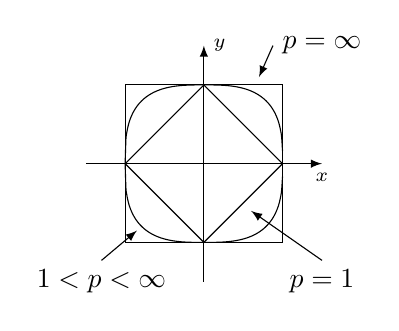
\begin{tikzpicture}
				\draw[-latex] (-1.5, 0)--(1.5, 0) node[below] {{$\scriptstyle x $}};
				\draw[-latex] (0, -1.5)--(0, 1.5) node[right] {{$\scriptstyle y $}};
				\draw (1, 1)-- ++(0, -2)-- ++(-2, 0)-- ++(0, 2)-- cycle;
				\node (pinfty) at (1.5, 1.5) {$ p=\infty $};
				\draw[-latex] (pinfty.west) -- (.7, 1.1);
				\draw (1, 0) -- (0, -1) --(-1, 0) -- (0, 1) -- cycle;
				\node (p1) at (1.5, -1.5) {$ p=1 $};
				\draw[-latex] (p1.north) -- (.6, -.6);
				\draw[smooth, samples=100, domain=0:1]plot(\x, {(1-(\x)^3)^(1/3)});
				\draw[smooth, samples=100, domain=-1:0]plot(\x, {(1+(\x)^3)^(1/3)});
				\draw[smooth, samples=100, domain=0:1]plot(\x, {-(1-(\x)^3)^(1/3)});
				\draw[smooth, samples=100, domain=-1:0]plot(\x, {-(1+(\x)^3)^(1/3)});
				% \draw plot (\x, {(cos(\x r))^(1/3)});
				\node (1pinfty) at (-1.3, -1.5) {$ 1<p<\infty $};
				\draw[-latex] (1pinfty.north) -- (-.85, -.85);
			\end{tikzpicture}
		\end{center}
	\end{minipage}\\